%
% Report: Verilog-A Macromodel for Resistive Potentiometers
%
% Copyright (C) 2008 Mike Brinson <mbrin72043@yahoo.co.uk>
%
% Permission is granted to copy, distribute and/or modify this document
% under the terms of the GNU Free Documentation License, Version 1.1
% or any later version published by the Free Software Foundation.
%

\documentclass[12pt,a4paper,oneside]{report}

% Include basic and title page definitions.
%
% This document contains a generic preamble for tutorials.
%
% Copyright (C) 2005 Stefan Jahn <stefan@lkcc.org>
%
% Permission is granted to copy, distribute and/or modify this document
% under the terms of the GNU Free Documentation License, Version 1.1
% or any later version published by the Free Software Foundation.
%

% Load some packages.
\newcommand{\tutpackages}{%
  \usepackage{savesym}
  \usepackage{a4wide}
  \usepackage[T1]{fontenc}
  \usepackage{longtable}
  \usepackage{ae,aecompl}
  \usepackage{url}
  \usepackage{epsfig}
  \usepackage{array}
  \usepackage{subfigure}
  \usepackage{amsmath}
  \usepackage{amsfonts}
  \usepackage{verbatim}
  \usepackage{fancyvrb}
  \savesymbol{iint}
  \usepackage{stmaryrd}
  \usepackage{wasysym}
  \restoresymbol{WASY}{iint}
  \usepackage{pifont}
  \usepackage[amssymb]{SIunits}
  \usepackage{graphics}
  \usepackage{psfrag}
  \usepackage{relsize}
  \usepackage[section]{placeins}
  \usepackage{listings}
  \iftutbook
  \else
    \usepackage{makeidx}
    \makeindex
  \fi
}

% Compatibility code for LaTeX and pdfTeX.
\newcommand{\tutcompat}{%
  \newif\ifpdf
  \ifx\pdfoutput\undefined
    \pdffalse
  \else
    \pdfoutput=1
    \pdftrue
  \fi
}

% Only evaluated if run using pdfTeX.
\newcommand{\tutheader}[2]{%
  \ifpdf
    \usepackage[pdftex,
	a4paper,
	backref,
	\iftutbook
	  anchorcolor=black,
	  filecolor=black,
	  menucolor=black,
	  pagecolor=black,
	  bookmarks=true,
	  bookmarksopen=true,
	  bookmarksnumbered=true,
	  pdfpagemode=UseOutlines,
	\else
	  bookmarks=false,
	  bookmarksopen=false,
	  bookmarksnumbered=true,
	  pdfpagemode=UseNone,
	\fi
	baseurl={http://qucs.sourceforge.net},
	pdfstartview=FitH,
	pdftitle={Qucs - \tuttitle},
	pdfauthor={#2},
	pdfsubject={#1},
	colorlinks,
	linkcolor=black,
	urlcolor=black,
	citecolor=black,
	backref=false,
	plainpages=false,
	pagebackref=false]{hyperref}
    \DeclareGraphicsExtensions{.pdf,.png}
    \pdfcompresslevel 9
    \pdfinfo {
      /Title   (Qucs - \tuttitle)
      /Subject (#1)
      /Author  (#2)
    }
  \else
    \DeclareGraphicsExtensions{.eps}
  \fi
  \graphicspath{{pics/}}
}

% Generic tutorial startup code.
\newcommand{\tutstartup}[2]{%
  \tutpackages
  \tutcompat
  \tutheader{#1}{#2}
}

% Begin document.
\newcommand{\tutbegin}{%
  \begin{document}
  \tuttitlepage
  \setlength{\parindent}{0pt}
}

% End document.
\newcommand{\tutend}{%
  \end{document}
}

%
% This document contains a generic title page for tutorials.
%
% Copyright (C) 2005, 2006 Stefan Jahn <stefan@lkcc.org>
%
% Permission is granted to copy, distribute and/or modify this document
% under the terms of the GNU Free Documentation License, Version 1.1
% or any later version published by the Free Software Foundation.
%

% Title page definitions.
\newcommand{\tuttitlepage}{%
  \makeatletter
  \begin{titlepage}
    \setlength{\parindent}{0pt}
    \vspace*{3cm}
    \begin{flushleft}
      \textbf{\begin{huge} Qucs \end{huge}}
    \end{flushleft}
    \hrule height 3pt
    \begin{flushright}
      \begin{LARGE} \tuttitle\\ \end{LARGE}
      \if\empty\tutsubtitle\else
        \vspace*{12pt}
        \begin{Large} \tutsubtitle \end{Large}
      \fi
    \end{flushright}
    \vfill
    \begin{flushright}
      \begin{Large} \tutauthor \end{Large}
    \end{flushright}
    \hrule height 3pt
    \vspace*{24pt} \tutcopyright \vspace*{12pt}

Permission is granted to copy, distribute and/or modify this document
under the terms of the GNU Free Documentation License, Version 1.1 or
any later version published by the Free Software Foundation.  A copy
of the license is included in the section entitled "GNU Free
Documentation License".

    \vspace*{1cm}
  \end{titlepage}
  \setcounter{footnote}{0}
  \makeatother
}

% Extra command for tutorial definitions.
\newcommand{\tutauthor}[1]{\def\tutauthor{#1}}
\newcommand{\tutcopyright}[1]{\def\tutcopyright{#1}}
\newcommand{\tuttitle}[1]{\def\tuttitle{#1}}
\newcommand{\tutsubtitle}[1]{\def\tutsubtitle{#1}}

% WorkBook conditional.
\newif\iftutbook
\tutbookfalse

% Section redefinitions.
\newcommand{\tutsection}[1]{%
  \iftutbook
    \section{#1}
  \else
    \section*{#1}
  \fi
}
\newcommand{\tutsubsection}[1]{%
  \iftutbook
    \subsection{#1}
  \else
    \subsection*{#1}
  \fi
}
\newcommand{\tutsubsubsection}[1]{%
  \iftutbook
    \subsubsection{#1}
  \else
    \subsubsection*{#1}
  \fi
}
\newcommand{\tutparagraph}[1]{%
  \iftutbook
    \paragraph{#1}
  \else
    \paragraph*{#1}
  \fi
}
\newcommand{\tutsubparagraph}[1]{%
  \iftutbook
    \subparagraph{#1}
  \else
    \subparagraph*{#1}
  \fi
}


\tuttitle{
  A Report}
\tutsubtitle{
  Verilog-A Macromodel for Resistive Potentiometers}
\tutauthor{
  Mike Brinson}
\tutcopyright{
  Copyright \copyright{} 2008 Mike Brinson
  \textless mbrin72043@yahoo.co.uk\textgreater}
\tutbookfalse

\tutstartup{\tutsubtitle}{Mike Brinson}

% Here finally starts everything.
\tutbegin

%
% Tutorial -- Component, compact device and circuit modelling
%             using symbolic equations
%
% Copyright (C) 2007 Mike Brinson <mbrin72043@yahoo.co.uk>
%
% Permission is granted to copy, distribute and/or modify this document
% under the terms of the GNU Free Documentation License, Version 1.1
% or any later version published by the Free Software Foundation.
%

% redefine subfigure caption
\renewcommand{\thesubfigure}{\thefigure(\alph{subfigure})}
\makeatletter
  \renewcommand{\@thesubfigure}{\thesubfigure:\space}
  \renewcommand{\p@subfigure}{}
\makeatother

% redefine subtable caption
\renewcommand{\thesubtable}{\thetable(\alph{subtable})}
\makeatletter
  \renewcommand{\@thesubtable}{\thesubtable:\space}
  \renewcommand{\p@subtable}{}
\makeatother

\tutsection{Introduction}

Qucs releases 0.0.11 and 0.0.12 mark a turning point in the
development of the Qucs component and circuit modelling facilities.
Release 0.0.11 introduced component values defined by equations and
for the first time allowed subcircuits with parameters.  Release
0.0.12 extends these features to add model development using symbolic
equations that are similar to compact device code written in the
Verilog-A modelling language. In designing the latest Qucs modelling
features the Qucs team has made a central focus of their work the need
to provide the package with an interactive and easy to use modelling
system which allows fast model prototype construction.  Much of these
new aspects have up to now been undocumented and are likely to be very
new to most Qucs users.  The aim of this tutorial note is to outline
the background to these important package extensions and to provide
real help to Qucs users who are interested in writing and
experimenting with their own models. The text includes a number of
illustrative examples for readers to try and experiment with.

\tutsection{Qucs electronic device and circuit modelling}

Circuit simulation packages are complex software systems which often
take years to mature to a stage where they are capable of analysing
the current generation of integrated and discrete electronic
circuits. Most circuit simulators have a number of common basic
attributes; firstly circuits are represented by a textual netlist or a
schematic diagram which contains all the information required by a
simulator to analyse the performance of a circuit, and secondly a
simulation engine which undertakes the calculation of circuit
performance in one or more different circuit domains such as DC, AC or
transient, and thirdly a post simulation processing system which
structures and displays the simulation data in both tabular and
graphical forms. All circuit simulators have one other important
attribute, namely that they represent individual electronic components
by a model, or abstraction, in a way that can be understood and
analysed by the simulation engine when undertaking a simulation
task. Without component models the science of circuit simulation would
not have developed to the stage it has today. From a users point of
view component models are the key to simulator productivity; the
greater the number of different models the easier it becomes to
analyse mixed analogue and digital electronic systems.

\vspace{5mm}
Shown in Fig.~\ref{fig:equ_1} is a block diagram of the analogue
component modelling and simulation facilities currently provided by
the Qucs package.  The diagram is structured as a flow chart which
emphasises the different device modelling routes.  When Qucs was first
released only two of these were available for users to develop new
device models.  The first of these has been used extensively by the
package developers to construct the built-in models that are
distributed with each Qucs release.  This fundamental route involves
hand coding the C++ code for a new model\footnote{The technical
details of the built-in models are described in: Qucs Technical
Papers, Stefan Jahn, Michael Margraf, Vincent Habchi and Raimund
Jacob, \url{http://qucs.sourceforge.net/technical.html}.}, its
compilation and linking with the core Qucs C++ code. Obviously, this
does require a specialised knowledge of the Qucs model programming
interface\footnote{Writing the documentation for the Qucs model
programming interface is on the to do list and will be completed, when
time allows, sometime in the future.}, the necessary C++ skills,
including a good working knowledge of the Trolltech Qt
toolkit\footnote{Qt is a registered trademark of Trolltech, Norway;
\url{http://www.trolltech.com/copyright}.}. At the time of writing these
notes the latest device to be added to Qucs using this approach is the
exponential pulse source\footnote{Added by Gunther Kraut on 15 April
2007. This device has been added for compatibility with
SPICE.}. Models based on hand written C++ code are normally restricted
to basic devices that form the fundamental component core of a
simulator - particularly where simulation computational efficiency is
important.  One disadvantage of this approach, is the obvious one, in
that the time to implement a new model increases disproportionately
with increasing model complexity.  For most Qucs users this route
would not be the most natural to use when developing new models.
However, for the specialist who spends a significant amount of time
researching new device models this has always in the past, been the
route of choice.  Unfortunately, modern semiconductor device models
are becoming so complex that the model development time can stretch
into months or even years and requires typically thousands of lines of
C or C++ code to characterise a model\footnote{A good introduction to
writing compact device models is given in ``How to (and how not to)
write a compact model in Verilog-A'', Geoffrey J. Coram, 2004,
Proc. 2004 IEEE International Behavioral Modeling and Simulation
Conference (BMAS 2004), pp 97- 106.}.  With the more complex models
the problem of finding bugs in the model code also acts as a limit to
fast model development.


\begin{figure}
  \centering 
  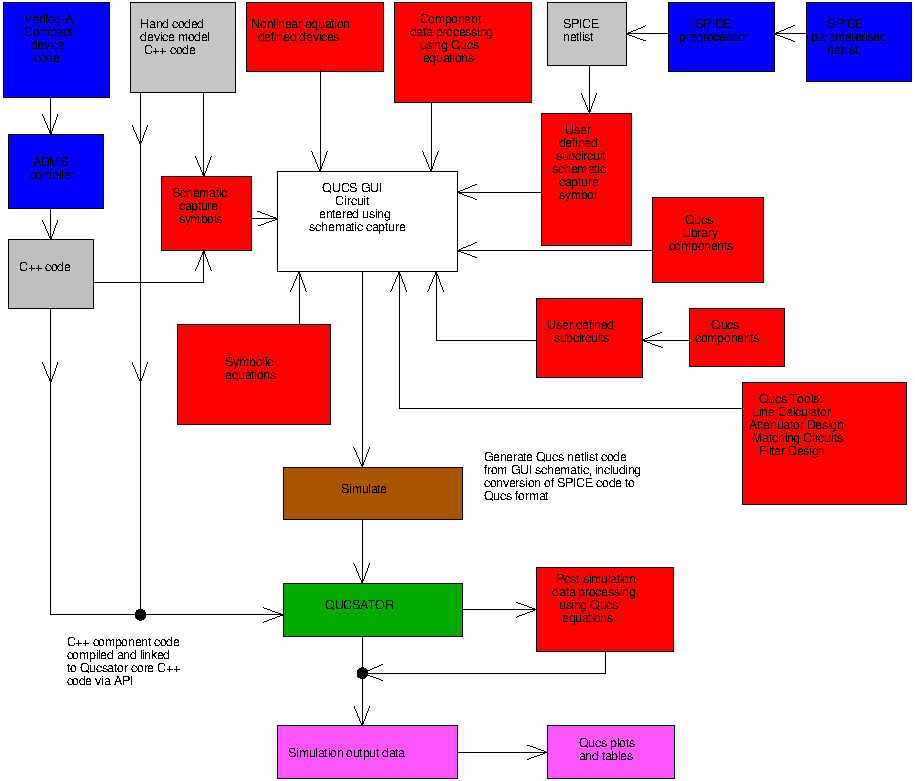
\includegraphics[width=1.0\linewidth]{equ_fig1a}
  \caption{Qucs analogue component modelling and simulation block diagram (not including optimisation)}
  \label{fig:equ_1}
\end{figure} 

\vspace{5mm}
For the average Qucs user their first introduction to the software is
probably through constructing circuit schematics made entirely from
the standard component models built into the package and the testing
of their performance by launching the simulator from one of the Qucs
simulation icons.\footnote{The ``Getting Started with Qucs'' tutorial
by Stefan Jahn outlines a number of basic simulation techniques;
\url{http://qucs.sourceforge.net/docs.html}.}  The next natural stage
in the Qucs modelling and simulation learning curve is the use of
subcircuits where groups of built-in components are collected together
to form a higher level circuit block.  These blocks are often arranged
with a common theme, forming a Qucs library. The process of modelling
new devices/circuits is normally done by connecting existing component
models and user defined subcircuits. With this type of modelling
higher level functional models can only be constructed from existing
fundamental components or previously constructed
subcircuits. Engineers often call this approach to modelling,
macromodelling.  Qucs releases up to 0.0.10 relied on macromodelling
for functional model development via the Qucs schematic interface.
This route remains popular amongst most Qucs users because it is easy
to understand, is fully interactive and allows straight forward
testing of new models. One feature that is common to all components
included in Qucs releases up to 0.0.10 may not be immediately obvious
to readers, namely that, with the exception of sweep variables,
component values could only be numbers, for example R1 = 1k, and were
not allowed to be represented by algebraic expressions like R1 =
Value1, where Value1 = 100.0+50\cdot X.  Its also worth pointing out
at this point that during simulation, again performed by Qucs releases
up to 0.0.10, component values were required to remain constant and
could not be a function of the circuit variables such as voltage,
current or charge.

\vspace{5mm}

One way to remove the component value restrictions imposed by early
Qucs releases is to model devices and circuits using preprocessor
extended forms of the SPICE netlist language. Circuit design equations
can then be embedded in SPICE netlists and the calculation of
component values completed by the SPICE preprocessor. Both the SPICE
to Qucs and OP AMP tutorials\footnote{Qucs simulation of SPICE
netlists and Modelling Operational Amplifiers, Mike Brinson,
\url{http://qucs.sourceforge.net/docs.html}.} outline in detail the steps
required to merge circuit design and simulation in this way.  This
modelling route is a very important and powerful model development
tool. So much so that ongoing tests to identify how compatible Qucs is
with the industrial standard SPICE 2g6 and 3f5 syntax are currently
being undertaken as part of the Qucs development
schedule\footnote{Qucs: Report Book; SPICE to Qucs test reports, Mike
Brinson, \url{http://qucs.sourceforge.net/docs.html}.}. Although perfectly
viable as a model development tool the use of an extended SPICE
netlist language has a number of serious disadvantages, namely that
not all the Qucs built-in component models have equivalent SPICE
models and secondly text netlists are the only entry medium for
describing models.

\vspace{5mm} 

The previous paragraphs give a brief statement of the different
component modelling routes that were available up to release
0.0.11. Qucs 0.0.11 is very much a modelling water shed in that
symbolic equations were introduced for the calculation of component
values, previously equations were only allowed when structuring
simulation output data for post simulation listing or
plotting. Release 0.0.11 allows the following types of variable;
\begin{enumerate}
\item sweep variables,
\item equations left hand side,
\item component parameter's left hand side (e.g. R1.R),
\item subcircuit parameters and
\item simulation output data.
\end{enumerate}
With each Qucs release the number of
analysis functions, and other data processing features, included in
the Qucs equation set continues to expand\footnote{See Measurement
Expressions Reference Manual, Gunther Kraut and Stefan Jahn,
\url{http://qucs.sourceforge.net/docs.html}.}. From release 0.0.11
parameters are also allowed with subcircuits so that data can be
passed to a model. This allows generalised subcircuit/macromodels to
be developed for popular devices such as operational amplifiers.
Through the use of embedded design equations within subcircuits and
parameter passing it became possible to construct powerful models that
mix both circuit design procedures and the calculation of individual
component values.  Qucs 0.0.11 still imposed the restriction that
equations could not be functions of voltage, current or charge.



\vspace{5mm}

With the release of Qucs 0.0.12 the voltage, current and charge
restrictions imposed on equations will finally be relaxed. The
introduction of a new device modelling component called the equation
defined device (EDD) allows firstly device current to be formulated as
a function of voltage, and secondly device charge to be calculated as
a function of voltage and current.  The syntax adopted for the new
model borrows heavily on the compact device modelling approach taken
by the Verilog-A modelling language.

\vspace{5mm}

Some readers will probably have noted that so far these notes make no
reference to the ADMS model development route illustrated in
Fig.~\ref{fig:equ_1}. ADMS stands for Automated device model
synthesizer\footnote{L.Lemaitre, C.C. McAndrew, and S. Hamm, ADMS -
Automated Device Model Synthesizer, Proc. IEEE CICC, 2002.} and
includes a Verilog-A to C/C++ compiler. It allows compact device
models to be described in the Verilog-A language then compiled to
C/C++ and the resulting code linked with the Qucs core simulation
code\footnote{For more details see, Qucs Description: Verilog-AMS
interface, Stefan Jahn and H\'{e}l\`{e}ne Parruitte,
\url{http://qucs.sourceforge.net/docs.html}.}. Model development using
ADMS is similar to the fundamental hand coded C++ model development
route except that model development is greatly simplified by the power
of the high level Verilog-A language.  A strong relationship exists
between the ADMS and EDD modelling procedures in that EDD can be
considered a fast interactive model prototyping method whose equations
can easily be expressed in Verilog-A and compiled into C/C++ code for
permanent inclusion in the Qucs simulator\footnote{Appendix A gives an
operator and function comparison table for Qucs and Verilog-A.}.

\vspace{5mm}

The opening paragraphs attempt to outline the available device
modelling techniques that are central to the functioning of the Qucs
package. The remaining sections of this tutorial note are devoted to
illustrating the power of Qucs modelling through the introduction of a
number of illustrative examples.  Initially these start from a simple,
and hopefully familiar, point and then proceed to more complex
examples which present many of the concepts lightly touched upon in
the opening text.


\tutsection{Extending circuit simulation capabilities with equations}

Just adding component value calculations, via equations, to a circuit
simulator immediately increases the underlying design and simulation
capabilities way beyond that found in earlier generation
simulators. Consider the simple RC circuit shown in
Fig.~\ref{fig:equ_2}. Capacitor \textit{Cap} is stepped from 0.1\micro
F to 1.1\micro F and the small signal AC response of the network
calculated. In this example the values for both \textit{R1} and
\textit{Cap} are given as numeric values. The simulation test shows
the effect of stepping the value of one component through a series of
values and recording the effect of component changes on circuit
performance. In other words this is a classical circuit analysis use
of a circuit simulator. In a real design situation different data is
often required. Most designers would prefer to find the value of
\textit{Cap} that gives a specific RC cut-off frequency ($f_{c}$) for
a specified value of \textit{R1}. This is the type of investigative
problem where adding equations into the simulation process generates
more informative results. Shown in Fig.~\ref{fig:equ_3} is a similar
RC network to that illustrated in Fig.~\ref{fig:equ_2}.

Capacitor voltage $VCap$ is given by:
\begin{equation}
V_{Cap}=\dfrac{V_1}{\sqrt{1+\omega^{2}\cdot C_1^{2} \cdot R_1^{2}}}
\end{equation}
where the cut-off frequency in the voltage transfer function is 
\begin{equation}
f_{c}=\dfrac{1}{2 \pi \cdot R_1 \cdot C_1}
\end{equation}

Hence, by expressing \textit{Cap} as a function of $f_{c}$ and
stepping $f_{c}$ through a range of frequencies, the effect of
capacitance changes on the voltage transfer function can be
found. More importantly a nomogram of \textit{Cap} values against
$f_{c}$ can be plotted giving the circuit designer a visual aid for
determing the value of \textit{Cap} required for given values of
\textit{R1} and $f_{c}$. Although the circuits shown in
Figs.~\ref{fig:equ_2} and~\ref{fig:equ_3} are very basic they do
demonstrate how much more powerful a circuit simulator becomes when
component values are calculated using equations.
 
\begin{figure}
  \centering
  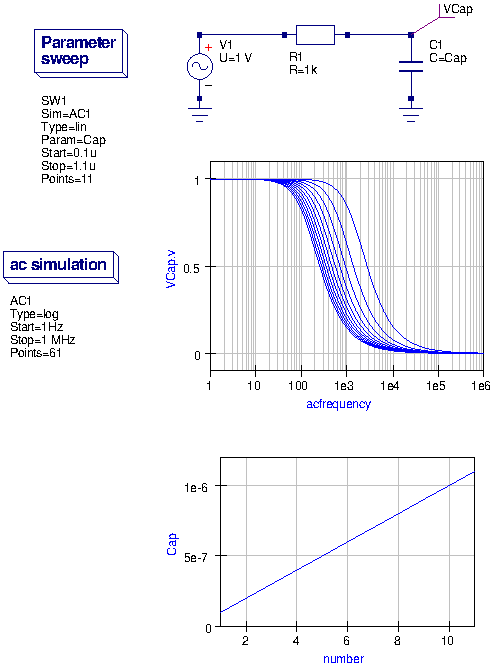
\includegraphics[width=0.9\linewidth]{equ_fig2}
  \caption{A simple RC circuit simulation using numerical component values}
  \label{fig:equ_2}
\end{figure} 

\begin{figure}
  \centering
  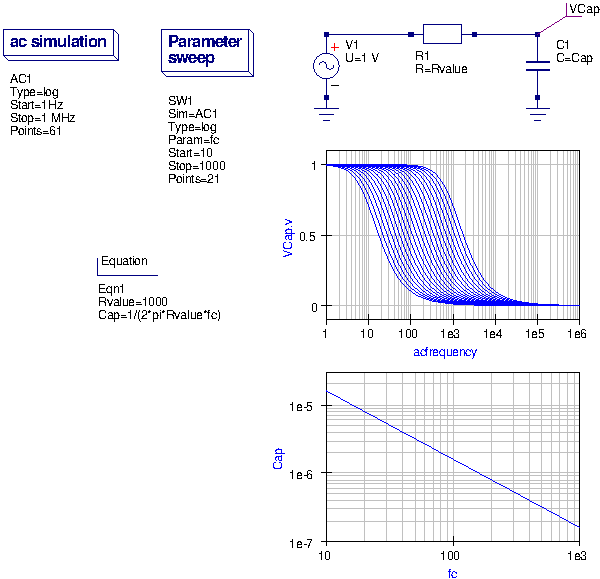
\includegraphics[width=1\linewidth]{equ_fig3}
  \caption{A simple RC circuit simulation employing equation determined component values}
  \label{fig:equ_3}
\end{figure} 

\tutsubsection{Low pass active filter design with embedded design equations}

In this section a more advanced circuit design example is introduced
to illustrate the power of embedded design equations in a Qucs
simulation schematic. A second order Sallen-Key low pass filter is
employed for this task because it is so well known and most readers
are likely to have met it's design in the past.  A second order low
pass filter is represented by the voltage transfer function:

\vspace{3mm}
\begin{equation}
A(S)=\dfrac{V_{out}}{V_{in}}=\dfrac{A0}{\left(1+a_{2}\cdot S + b_{2}\cdot S^{2} \right) }
\end{equation}  

\vspace{3mm}

where $A0$ is the passband DC gain and coefficients $a_{2}$, $b_{2}$
are for Bessel, Butterworth, Tschebyscheff or similar polynomials.

\vspace{3mm}

The following list\footnote{See OP Amps for everyone, Chapter 16:
Active filter design technology, Texas Instruments, August 2002,
SL0D006B, PP 16.1,16.63.} gives the second order coefficients for the
Bessel $\rightarrow$ 1.3617, 0.618; Butterworth $\rightarrow$ 1.4142,
1.000; and 3dB ripple Tschebyscheff $\rightarrow$ 1.065, 1.9305,
polynomials. The second order Sallen-Key low pass filter circuit is
shown in Fig.~\ref{fig:equ_4}. This circuit has a voltage gain
transfer function given by:

\vspace{3mm}

\begin{equation}
A(S)=\dfrac{A0}{1+\omega_{c}\cdot\left[ C_{1}\cdot \left(R_{1}+R_{2}\right)+\left(1-A0\right)\cdot R_{1}\cdot C_{2}\right]\cdot S+\omega_{c}^{2}\cdot R_{1}\cdot R_{2}\cdot C_{1}\cdot C_{2}\cdot S^{2}}
\end{equation}
where
\begin{equation}
A0=1+\dfrac{R_{3}}{R_{4}} 
\end{equation} 

This can be simplified by letting $R_{1}=R_{2}=R$ and $C_{1}=C_{2}=C$;
the transfer function then becomes:

\begin{equation}
A(S)=\dfrac{A0}{1+\left[ \omega_{c}\cdot R\cdot C\cdot\left(3-A0\right)\right]\cdot S+\left[ \left(\omega_{c}\cdot R\cdot C\right)^{2}\right]\cdot S^{2}}.\end{equation}

By comparison  
\begin{equation}
a_{2}=\omega_{c}\cdot R\cdot C\cdot \left(3-A0\right)
\end{equation}
 and  
\begin{equation}
b_{2}=\left(\omega_{c}\cdot R\cdot C\right)^{2}
\end{equation}

Fixing $C$ and solving for $R$ and $A0$, yields
\begin{equation}
R=\dfrac{\sqrt{b_{2}}}{\omega_{c}\cdot C}
\textrm{ , and }
A0=3-\dfrac{a_{2}}{\sqrt{b_{2}}}.
\end{equation}
Also once A0 is known the value for $R4$ can be calculated using
equation
\begin{equation}
A0=1+\dfrac{R3}{R4}.
\end{equation}
Hence by providing values for $C$ and $R3$ the values for $R$ and
$A0$, and of course $R4$, can be determined for a specified cut off
frequency $fc$. Figure~\ref{fig:equ_5} shows the final design
schematic and the simulation results for this example. A number of
important observations can be made from Fig.~\ref{fig:equ_5}:

\begin{figure}
  \centering
  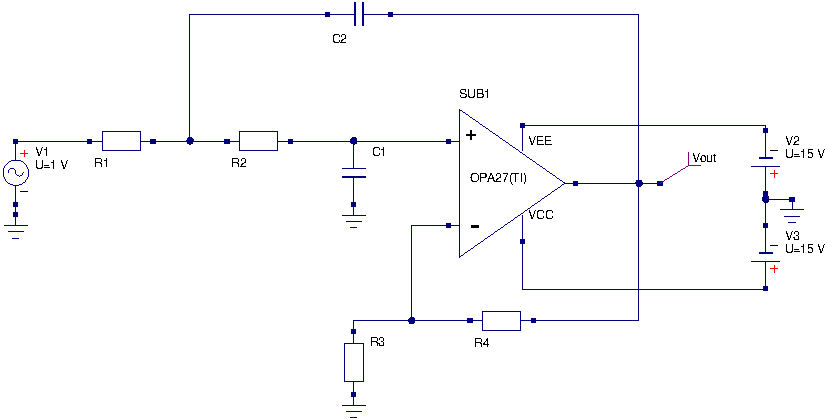
\includegraphics[width=1\linewidth]{equ_fig4}
  \caption{The Sallen-Key lowpass active filter circuit}
  \label{fig:equ_4}
\end{figure} 

\begin{figure}
  \centering
  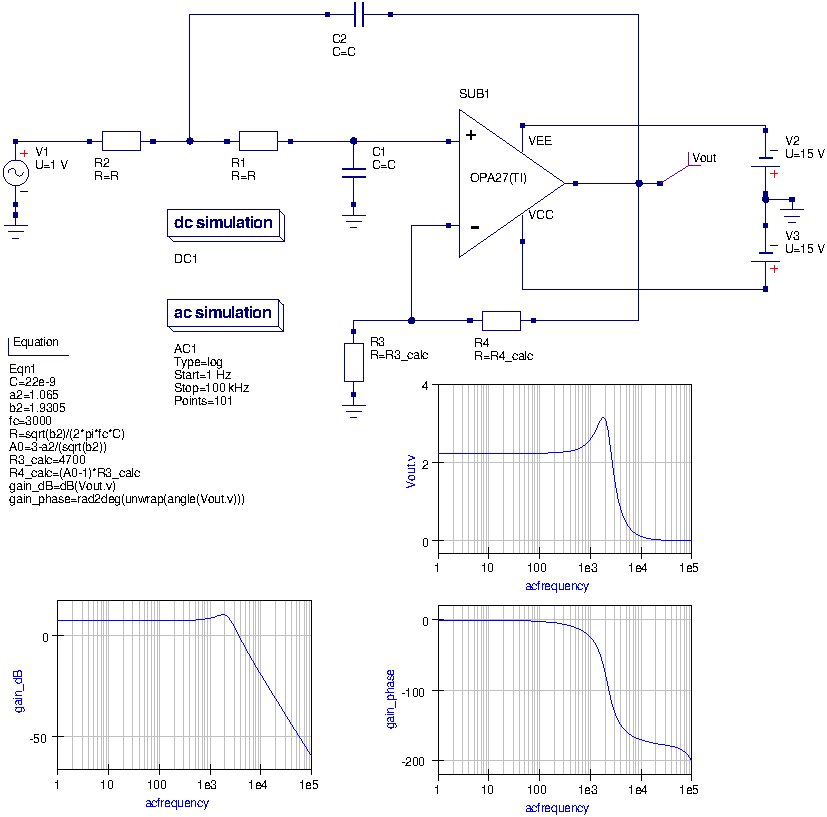
\includegraphics[width=1\linewidth]{equ_fig5}
  \caption{The Sallen-Key lowpass active filter schematic with embedded design equations}
  \label{fig:equ_5}
\end{figure} 
 
\begin{enumerate}
  \item One or more equation blocks hold both design and post
  simulation data processing equations plus assignments for named
  items: $C$, $fc$ and $R3$ are given numerical values, the a and b
  polynomial coefficients are set to the values introduced in the
  text, and finally the design equations for $R$, $A0$ and $R4$
  calculations are listed.

  \item The order of entries in equation blocks is not important
  because Qucs automatically sorts out the data it requires when
  calculating equations.

  \item The lefthand quantities in the assignment entries in the
  equation blocks are linked to the component values in the schematic,
  see for example $C$ and $R$.

  \item The OP27 operational amplifier model is from the modified Qucs
  0.0.11 OPAMP library. This model was generated using the SPICE to
  Qucs modelling route.

  \item To design and simulate a Sallen-Key low pass filter with a
  different cut off frequency\footnote{If the design calculations
  result in impractical values for the filter components then the
  value of C should be changed and the simulation repeated.} simply
  change the value of $fc$ and rerun the Qucs simulator.

  \item On completion of a simulation, pressing key F5 (Show last
  messages) causes the simulation log to be displayed. This includes
  the calculated values of the components and the netlist for the
  circuit, see Fig.~\ref{fig:equ_6}.

  \item One final point of significance that some readers may have
  noticed - all numerical values in equation blocks must be specified
  in scientific notation; electronic notation like 1k or 3nF is not
  allowed\footnote{In long term it is expected that electronic
  notation will be allowed. The changes for this are on the to do list
  but at the moment the work has a low priority.}.
\end{enumerate}





\begin{figure}
  \centering \begin{lstlisting}[ language=Clean, basicstyle = \small ]
Output:
-------
netlist content
  13 R instances
   5 C instances
   2 VCCS instances
   5 CCCS instances
   2 VCVS instances
   1 CCVS instances
   8 Vdc instances
   1 Idc instances
   1 Vac instances
   4 Diode instances
   2 BJT instances
   1 DC instances
   1 AC instances
creating netlist...
checker notice, variable `Vout.v' in equation `gain_dB' not yet defined
checker notice, variable `Vout.v' in equation `gain_phase' not yet defined
kB = 1.38065e-23
e = 2.71828
pi = 3.14159
C = 2.2e-08
a2 = 1.065
b2 = 1.9305
fc = 3000
R = 3350.51
A0 = 2.2335
R3_calc = 4700
R4_calc = 5797.43
kB = 1.38065e-23
e = 2.71828
pi = 3.14159
kB = 1.38065e-23
e = 2.71828
pi = 3.14159
kB = 1.38065e-23
e = 2.71828
pi = 3.14159
\end{lstlisting}

  \caption{Message output log for the simulation of the Sallen-key low pass circuit: for brevity only the component value section is given}
  \label{fig:equ_6}
\end{figure} 
 
\tutsection{Introduction to Qucs subcircuit parameters}

Subcircuits are a concept that has been part of the simulation scene
for a long time. All circuit simulators based on SPICE have
subcircuits as part of their basic device compliment. This is not
surprising because they form a natural way of breaking an electronic
system down into a number of smaller self contained functional blocks.
What is surprising however, is the fact that a significant number of
simulators, including SPICE 2g6 and 3f5\footnote{One of the reasons
SPICE preprocessors were developed was to allow parameter passing to
subroutines, for more details see Qucs Tutorial: Qucs simulation of
SPICE netlists, Mike Brinson, \url{http://qucs.sourceforge.net/}.}, do
not allow parameters to be passed to a subcircuit.  Parameter passing
appears to have been first introduced when a number of the popular
commercial circuit simulators were being developed\footnote{See, for
example, the extended netlist format originally designed by the
MicroSim Corporation for the PSpice circuit simulator. }.  Qucs
releases up to version 0.0.10 are similar to SPICE in that they also
did not allow parameters with subcircuits.

\vspace{3mm}
This very important limitation has been removed with release 0.0.11,
which allows parameters to be attached to component symbols and used
in subcircuit equation calculations.  Shown in Fig.~\ref{fig:equ_7}
are the circuit schematic and user generated symbol for a simple
harmonic generator with a fundamental and three harmonic sinusoidal
components. Parameters \textit{f1} to \textit{f4} determine these
frequency components. Notice that an equation block, at the circuit
schematic level, is used to calculate the harmonic
frequencies. Parameters \textit{ph1} to \textit{ph4} set the phase of
the individual sinusoidal oscillators. The process of attaching
parameters, and their default values, to a subcircuit symbol is
straightforward; simply right click on the symbol subcircuit name,
\textit{SUB1} in Fig.~\ref{fig:equ_7}, and an Edit Subcircuit
Properties dialog box appears allowing parameter names and their
default values to be entered\footnote{See Appendix B for a more
detailed description of the procedure.}. Subcircuit parameters and
their values are normally displayed as a list underneath the
subcircuit name.  Changing parameter values is done in a similar
fashion to changing the values of the standard built-in
components. The diagram and simulation results illustrated in
Fig.~\ref{fig:equ_8} show a waveform formed from a fundamental and two
harmonics.

\vspace{3mm}
An equation block is employed to calculate and plot the amplitude and
power spectral densities of the harmonic waveform. By changing the
fundamental frequency, signal amplitudes and phases different wave
shapes can be generated by resimulating the circuit. In this example
transient analysis is used to generate the harmonic waveform with the
run time set to 10ms and the number of points equal to
500\footnote{Qucs function length() determines the correct data length
in equation block Eqn1 calculations.}. This gives a sampling time of
20\micro s and a sampling frequency of 50kHz. Equation block
\textit{Eqn1} demonstrates how the Qucs functions\footnote{If you have
used a program like Octave, or indeed Matlab, many of these functions
should be familiar to you. These functions provide Qucs with powerful
numerical resource which significantly extends the range of problems
that Qucs can analyse.} can be used to postprocess simulation
generated data - in this example they are used to compute the DFT of
the harmonic generator waveform, convert the resulting spectra from
double sided to single sided form, compute and plot the amplitude and
power spectral densities.

\begin{figure}
  \centering
  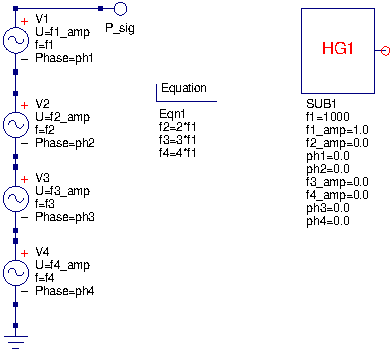
\includegraphics[width=0.6\linewidth]{equ_fig7}
  \caption{Harmonic generator subcircuit schematic and symbol} 
  \label{fig:equ_7}
\end{figure} 

\begin{figure}
  \centering
  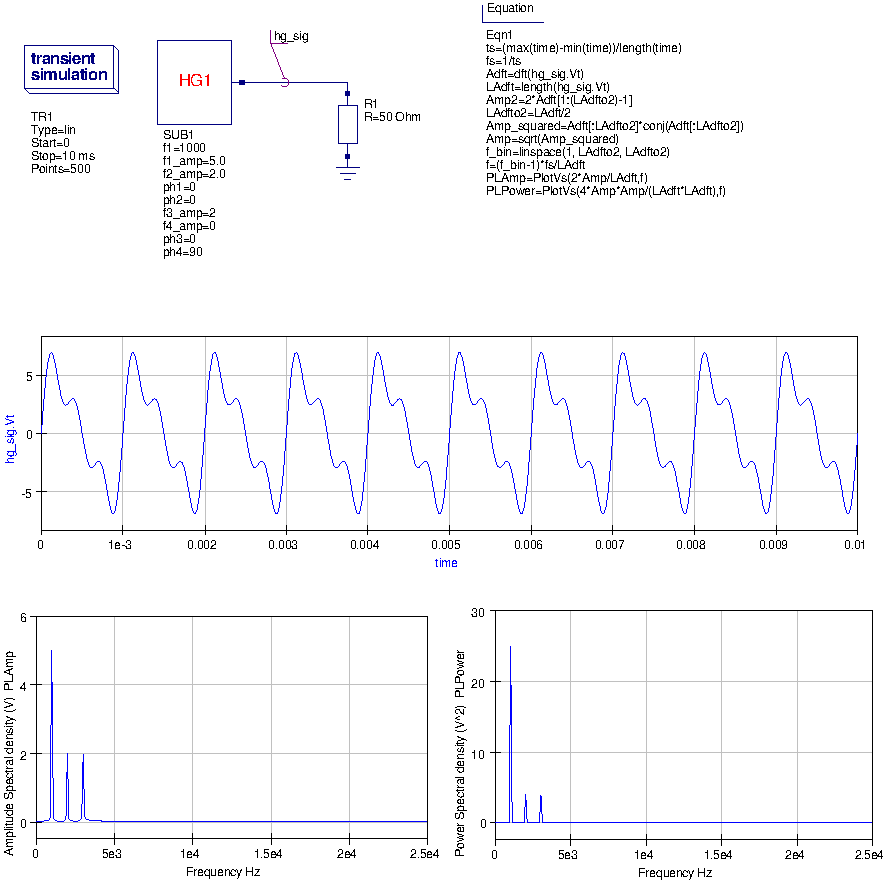
\includegraphics[width=1.1\linewidth]{equ_fig8}
  \caption{Harmonic generator subcircuit test circuit and simulation waveforms}
  \label{fig:equ_8}
\end{figure} 

\tutsection{Building universal macromodels using subcircuits and parameters}

Passing parameters to subcircuits allows universal macromodels to be
built. One obvious application of this technique is the modelling of
operational amplifiers (OP AMP) and other integrated circuits.  The
approach adopted is similar to that outlined in the last section.
However, because of the complexity of the models it is advisable to
break a model into a series of smaller blocks. These are then combined
to form a complete subcircuit macromodel. Two techniques are possible
when partitioning models, these are demonstrated next. Shown in
Fig.~\ref{fig:equ_8a} is a simple AC OP AMP model\footnote{The term AC
here refers to the fact that the OP AMP model chosen for demonstration
purposes is a simplified version of a multi-domain OP AMP model. It
only models small signal AC parameters and device input stage bias and
offset properties.} consisting of an input stage, an intermediate gain
stage and an output stage\footnote{The schematic shown in
Fig.~\ref{fig:equ_8a} forms part of a modular OP AMP macromodel. A
detailed description of the function of individual networks and the
derivation of the component equations is given in Qucs tutorial
Modelling Operational Amplifiers, Mike Brinson,
\url{http://qucs.sourceforge.net/docs.html}.}. An equation block, if needed,
is associated with each stage. These blocks contain the equations for
calculating the component values in a given stage. A single schematic
symbol represents the model. This has a list of parameters
attached. The flow of information into a macromodel starts with
parameters passed into a subcircuit, via a schematic symbol, then onto
the equation blocks, where it is finally used to calculate the
component values.  Hence, by simply changing the subcircuit parameters
different OP AMPs can be simulated using a single generalised
macromodel. However, please note that different OP AMP circuit
structures, or indeed technologies, naturally result in a series of
generalised subcircuit macromodels to cover all possible types in a
given device family.  The second technique involves breaking a model
down into smaller blocks and associating subcircuit symbols with each
block. This approach is illustrated in Fig.~\ref{fig:equ_8b}. Again
parameters are passed from the top level symbol (called AC in the
schematic) to the inner subcircuits. These pass their own parameters
down a subcircuit level where the component calculations are
completed. The second technique results in two levels of subcircuit,
accounting for the change in parameter name when passing a parameter
from top to lower hierarchy. A second more detailed example showing
how to construct nested subcircuits is presented later in these notes.

\begin{figure}
  \centering
  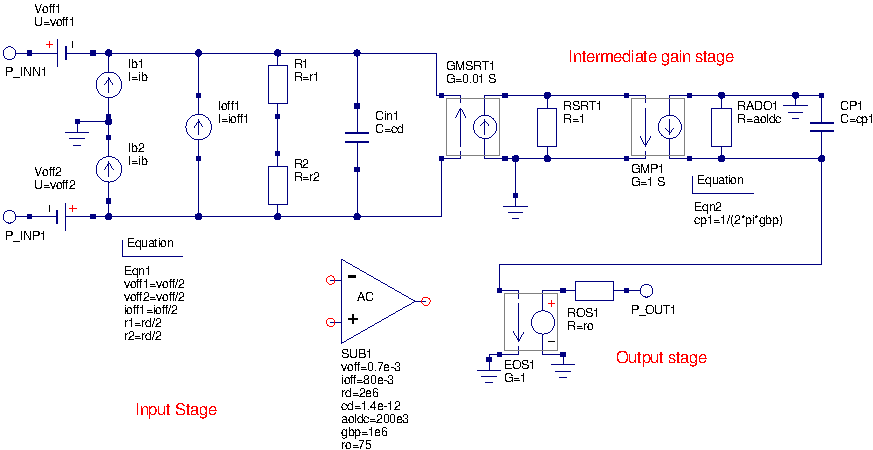
\includegraphics[width=1\linewidth]{equ_fig8a}
  \caption{Expanded AC OP AMP model showing circuitry and equation blocks} 
  \label{fig:equ_8a}
\end{figure} 


\begin{figure}
  \centering
  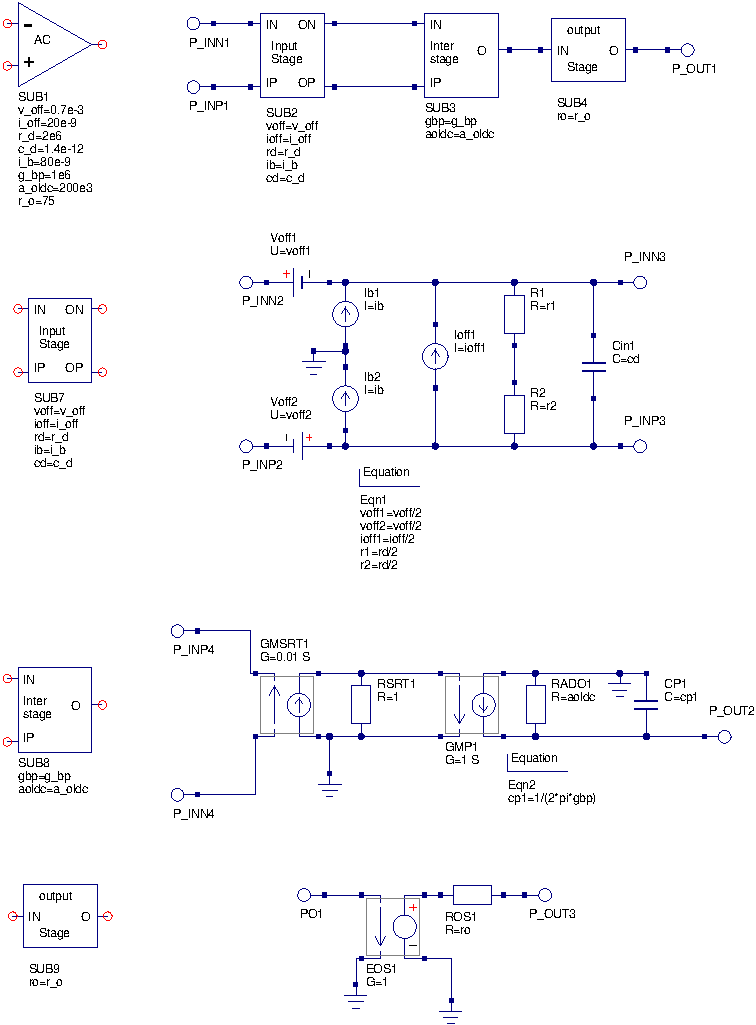
\includegraphics[width=0.9\linewidth]{equ_fig8b}
  \caption{Modular AC OP AMP model showing subcircuits}
  \label{fig:equ_8b}
\end{figure} 


\vspace{5mm}
In reality the macromodel for a typical OP AMP that models DC, AC and
transient domains is much more complex than the model given in
Fig.~\ref{fig:equ_8a}.  The schematic for a typical multi-domain OP
AMP modular macromodel is shown in Fig.~\ref{fig:equ_9}, where each
section of the macromodel is represented, if needed, by it's own
equation block.

 


\begin{figure}
  \centering
  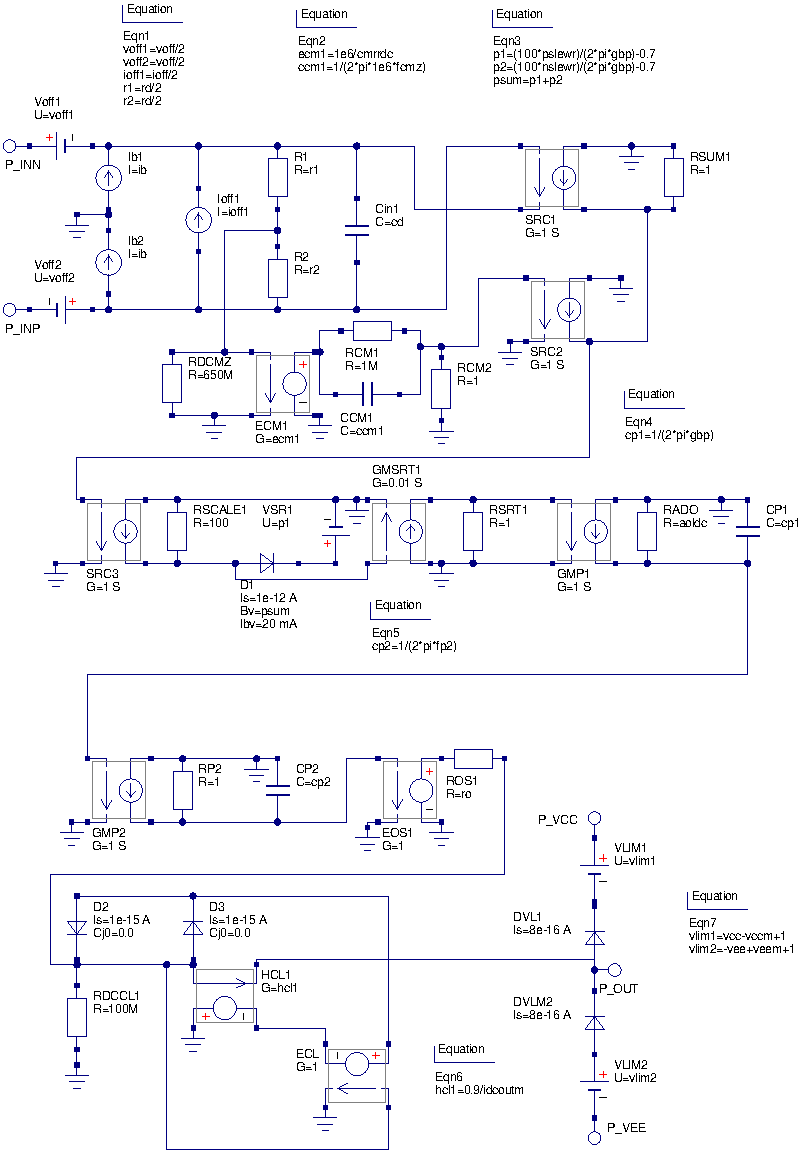
\includegraphics[width=0.9\linewidth]{equ_fig9}
  \caption{Modular OP AMP subcircuit schematic with embedded component calculation equations}
  \label{fig:equ_9}
\end{figure} 

\vspace{3mm}

The test schematics shown in Figures.~\ref{fig:equ_10}
and~\ref{fig:equ_11} show two OP AMPs with different subcircuit
parameters. In Fig.~\ref{fig:equ_10} the small signal characteristics
of unity gain closed loop amplifiers clearly show the difference in
performance of the OP AMPs.  Figure~\ref{fig:equ_11} is particularly
interesting in that it illustrates how Qucs can be used to determine
the effect of amplifier offset voltage on integrator DC saturation by
stepping resister \textit{rp} through a series of values. The low
offset voltage of the OP27 makes this device much more suitable for
integrator circuits when compared to the popular UA741. These results
can be confirmed by a simple calculation: the offset voltage for the
UA741 is set at $0.7$ mV and the amplifier open loop DC gain at
roughly $200,000$. The UA741 goes into saturation when \textit{rp} is
approximately 20 M$\Omega$. In saturation the OP AMP gain becomes open
loop giving a DC output voltage of roughly 0.7e-3\cdot 2e5 or $14$ V,
which agrees with the Qucs simulation results.


\begin{figure}[h]
  \centering
  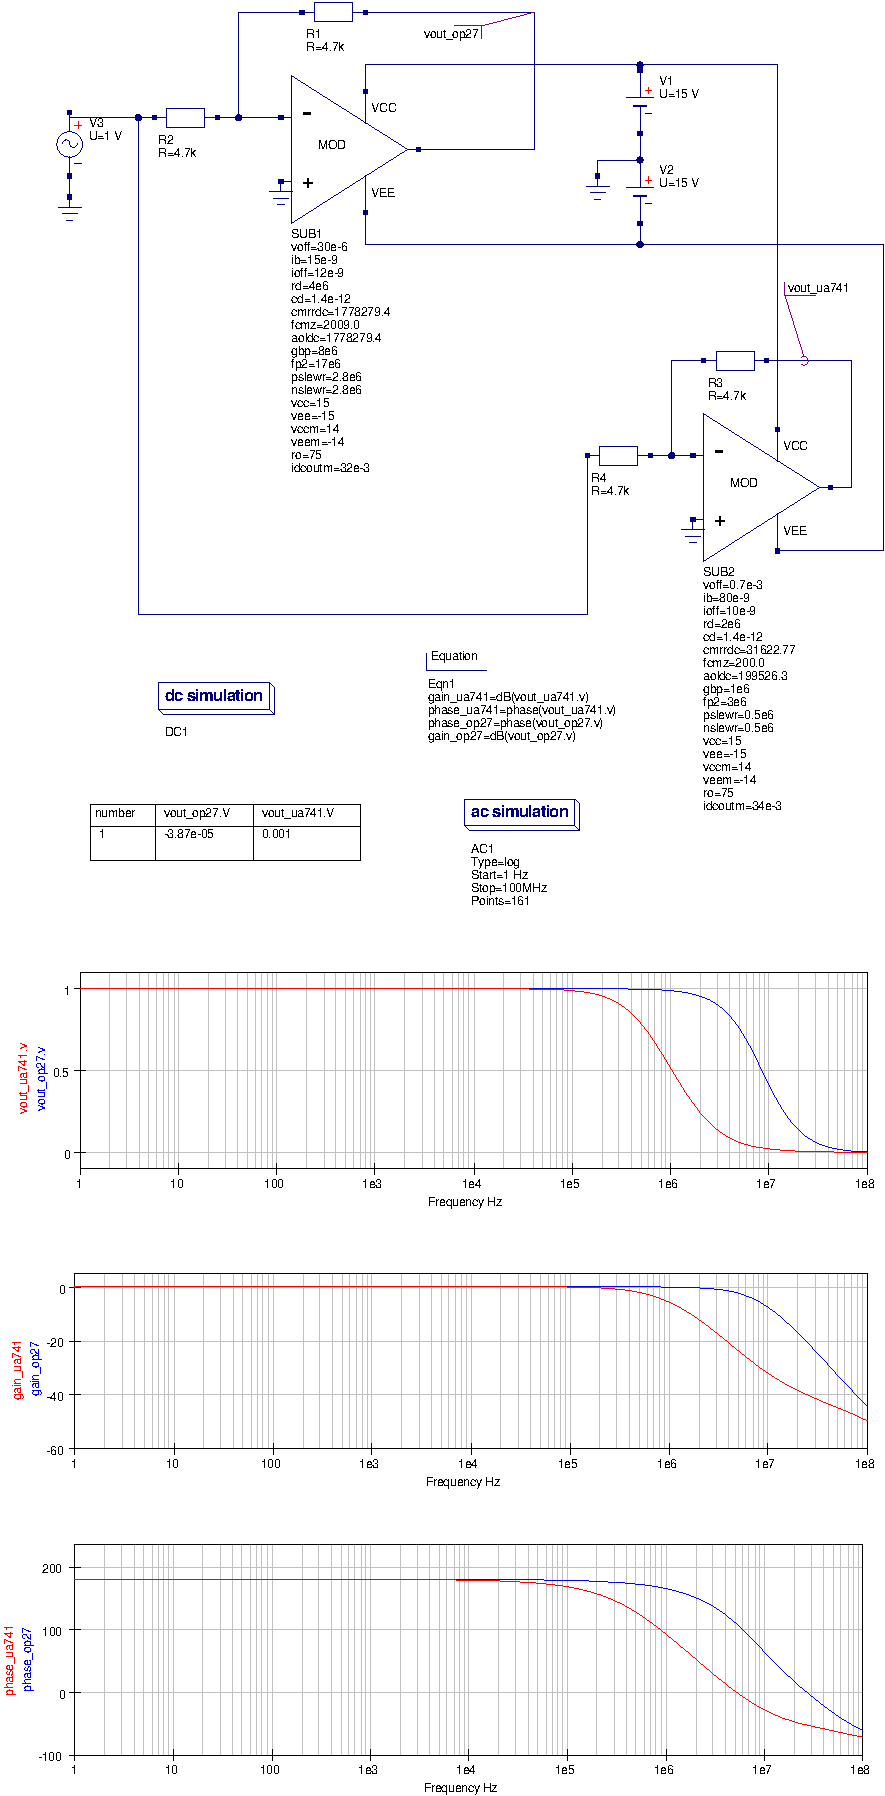
\includegraphics[width=0.65\linewidth]{equ_fig10}
  \caption{Unity gain OP AMP test circuit and waveforms} 
  \label{fig:equ_10}
\end{figure}  



\begin{figure} [h]
  \centering
  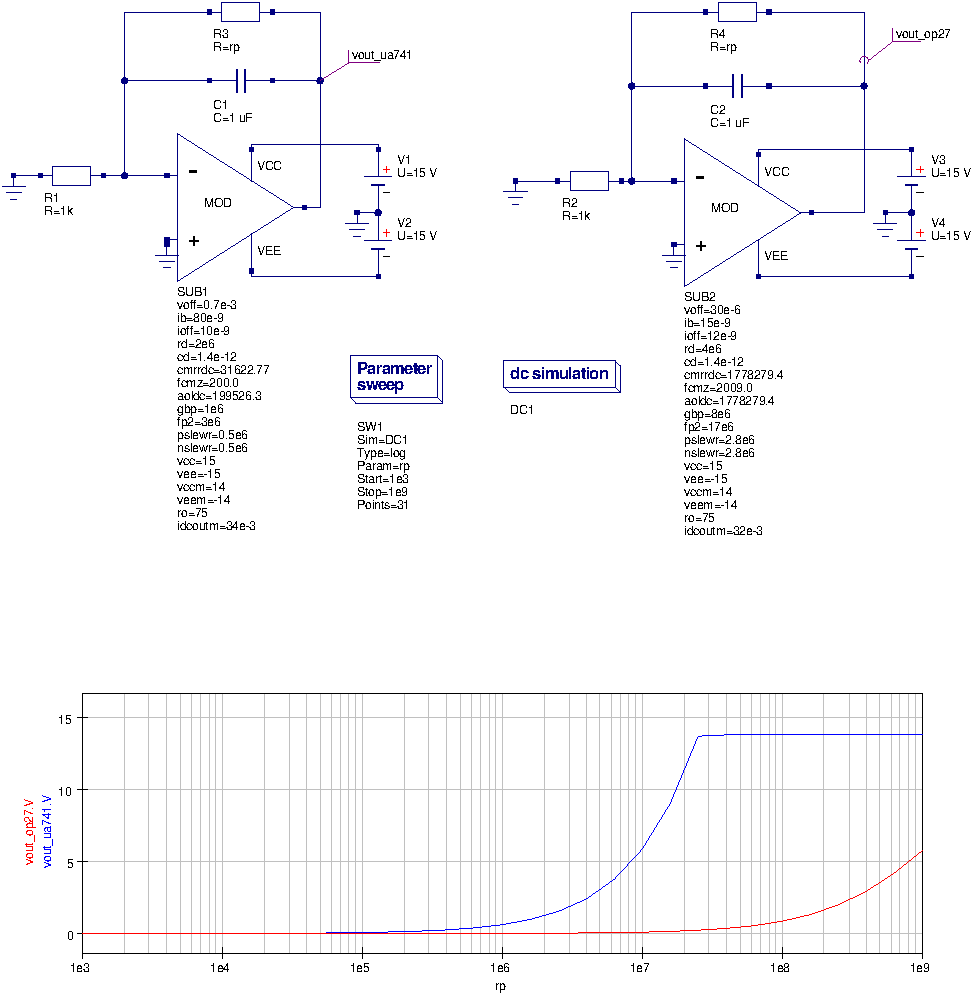
\includegraphics[width=1.0\linewidth]{equ_fig11}
  \caption{Integrator test circuits for determining DC saturation}
  \label{fig:equ_11} 
\end{figure} 

\tutsection{More complex nested subcircuit models}

In the previous two sections the example circuits only included
subcircuits nested to one or two levels. Qucs does however, allow
subcircuits to be nested to an arbitrary level and parameters can be
passed down the nested chain to any depth required. Some care is
needed when setting up the parameter passing sequence.  Shown in
Fig.~\ref{fig:equ_12} is a top level subcircuit with temperature swept
between 10 and 110 centigrade. A simple resistor voltage divider
network is at the bottom of a series of linked subcircuits, three
levels down. R2 in the divider is a function of temperature. A
schematic representation of the coupled subcircuits parameter passing
sequence is also given in the right hand side of
Fig.~\ref{fig:equ_12}. Each level passes the value of temperature to
it's next lower member in the hierarchy.  The Qucs generated netlist
given in Fig.~\ref{fig:equ_13} clearly shows the parameter passing
mechanism employed by Qucs.  The ability to nest subcircuits and pass
parameters down a hierarchy is an important feature in Qucs because it
allows both circuit design and device data to be passed to different
sections of the circuit/system being simulated.  These parameters can,
of course, be at different levels in a problem hierarchy providing a
very flexible and powerful design/analysis tool.


\begin{figure}[h]
  \centering
  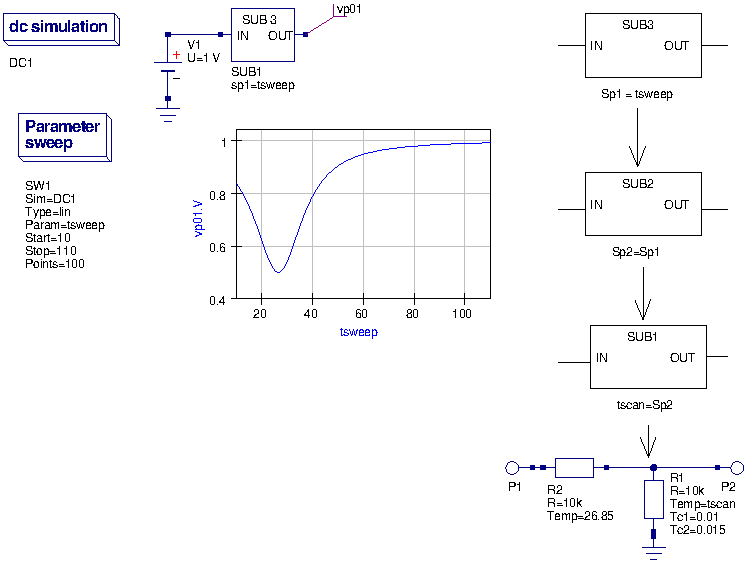
\includegraphics[width=0.9\linewidth]{equ_fig12}  
  \caption{A nested subcircuit showing parameter passing sequence }
  \label{fig:equ_12}
\end{figure} 

\begin{figure} [h]
  \centering 
 \begin{lstlisting}[
  language=Clean,
  basicstyle = \footnotesize]
# Qucs 0.0.12  /media/hda2/Qucs_equation_modelling_prj/rdiv_test_tsweep_3l.sch
.Def:rdiv_sub1_temp _net1 _net0 tscan="27"
R:R2 gnd _net0 R="10k" Temp="tscan" Tc1="0.01" Tc2="0.015" Tnom="26.85"
R:R1 _net1 _net0 R="10k" Temp="26.85" Tc1="0.0" Tc2="0.0" Tnom="26.85"
.Def:End

.Def:rdiv_test6_temp _net1 _net0 sp2="27"
Sub:SUB1 _net1 _net0 Type="rdiv_sub1_temp" tscan="sp2"
.Def:End

.Def:rdiv_sub3_temp _net0 _net1 sp1="27"
Sub:SUB1 _net0 _net1 Type="rdiv_test6_temp" sp2="sp1"
.Def:End

Vdc:V1 _net0 gnd U="1 V" 
.DC:DC1 Temp="26.85" reltol="0.001" abstol="1 pA" vntol="1 uV" 
saveOPs="no" MaxIter="150" saveAll="no" convHelper="none" Solver="CroutLU"
.SW:SW1 Sim="DC1" Type="lin" Param="tsweep" Start="10" Stop="110" Points="100"
Sub:SUB1 _net0 vp01 Type="rdiv_sub3_temp" sp1="tsweep"

\end{lstlisting}
  \caption{Qucs netlist for nested subcircuit showing parameter passing sequence}
  \label{fig:equ_13}
\end{figure} 



\tutsection{Introduction to equation defined devices (EDD)}

Although adding symbolic equations to a simulator merges circuit
design and analysis, it is by making these equations functions of
circuit variables that the real power of modern circuit simulator is
fully exploited. Equations that are functions of voltage, current and
charge have to be continuously evaluated as a simulation
progresses. This is in contrast to the type of equations previously
introduced, which are only evaluated at the start of a simulation
sequence.  When component properties are functions of circuit
variables considerable complexity is added to a simulation engine and
as a result most simulators restrict such properties to a small number
of component types, the most common being controlled current and
voltage generators\footnote{Probably the most well known non-linear
controlled generators are the SPICE 2g6 and 3f5 forms, see
A. Vladimirescu, Kaihe Zhang, A.R. Newton, D.O. Pederson and
A. Sangiovanni-Vincentelli, SPICE Version 2G User's Guide, 1981,
Department of Electrical Engineering and Computer Sciences, University
of California, Berkeley, Ca. 94720, section 11, Appendix B: Nonlinear
dependent sources., and B. Johnson, T. Quarles, A.R. Newton,
D.O. Pederson and A. Sangiovanni-Vincentelli, SPICE3 Version f User's
Manual, 1992, Department of Electrical Engineering and Computer
Sciences, University of California, Berkeley, Ca. 94720, section
3.2.2.4, Non-linear dependent sources.}. Qucs version 0.0.12
introduces an equation defined device (EDD) which allows it's terminal
currents to be functions of voltage, and it's stored charge to be
functions of voltage and current. The EDD is similar, but more
advanced, to the B type controlled source implemented in SPICE 3f5. It
is capable of realising the same models as the SPICE B type device
plus an extensive range of more complex compact device models. At this
stage in Qucs development only the explicit form of EDD is
implemented\footnote{See Qucs Technical Papers, Section 10.7: Equation
defined models, Stefan Jahn, Michael Margraf, Vincent Habchi and
Raimund Jacob, \url{http://qucs.sourceforge.net/technical.html}.}. EDD
is an advanced component that allows Qucs users to construct their own
device models from a set of equations derived from the physical
properties that characterise a device. The explicit form of EDD can
only be used to develop models for devices where their defining
equations can be transformed into the explicit analysis form required
by Qucs\footnote{The Y parameters of the device being modelled must
also exist for the explicit form of the EDD to be valid.}. A range of
functions similar to those defined in the Verilog-A compact device
modelling language are provided by Qucs, making the equation modelling
language easy to use and powerful. The ternary ? : form of the C
language if statement has also been implemented to allow selection of
model equations that change with differing device voltage, current and
charge conditions.  Before introducing the EDD symbol and it's
properties consider the following circuit simulation modelling
problem: a model for a device is required where the output voltage is
a function of two input voltages $VIN_1$ and $VIN_2$, such that

\begin{equation}
V_{out}\left(VIN_1,VIN_2\right) = VIN_1\cdot VIN_2,
\end{equation}

where $VIN_1$ and $VIN_2$ can be arbitrary varying voltages.

\vspace{3mm}

This type of model is difficult to simulate at functional
level\footnote{It is, of course, possible to model the multiplier
operation at discrete component level e.g. using a Gilbert cell mixer
circuit.} using the pre-version 0.0.12 built-in devices.  A linear
voltage controlled voltage source can be used to multiply a voltage by
a constant.  Multiplying by a second voltage is not possible with the
linear controlled sources. Qucs AM modulated and PM modulated sources
are the nearest that Qucs has to the source defined above. These
sources however, only allow sinusoidal carrier signals.  Illustrated
in Fig.~\ref{fig:equ_14} is a four quadrant multiplier EDD which
allows multiplication of two varying signals\footnote{This model is
based on an idea suggested by Stefan Jahn, during the EDD development
phase.}. The EDD device generates current $I1 = V2\cdot V3$. This in
turn is transformed to the output voltage by a unity gain current
controlled voltage source SRC1. An EDD device can consist of up to 8
branches. The branches have currents, I1 to I8, voltages V1 to V8 and
internal charges Q1 to Q8 respectively. Overall the total device
current depends how these branches are connected. A similar comment
applies to the total device charge. In Fig.~\ref{fig:equ_14} currents
I2 and I3 are set to zero, charges Q2 and Q3 are also zero, and
voltages $V2=VIN_1$ and $V3=VIN_2$. Hence current I1 becomes the
multiplication of $VIN_1$ and $VIN_2$. The fact that currents I2 and
I3 are set to zero implies that the terminals connected to the
external input voltages have high impedance and act as voltage
probes. The test circuit in Fig.~\ref{fig:equ_14} is shown with signal
inputs generated by sinusoidal oscillators; V1 acts as a modulating
signal and V2 as a carrier signal. The bottom right hand corner of
Fig.~\ref{fig:equ_14} includes a second graph which illustrates the
effect of changing signal V2 to a square wave source with 0.05ms
period.


\begin{figure}[h]
  \centering
  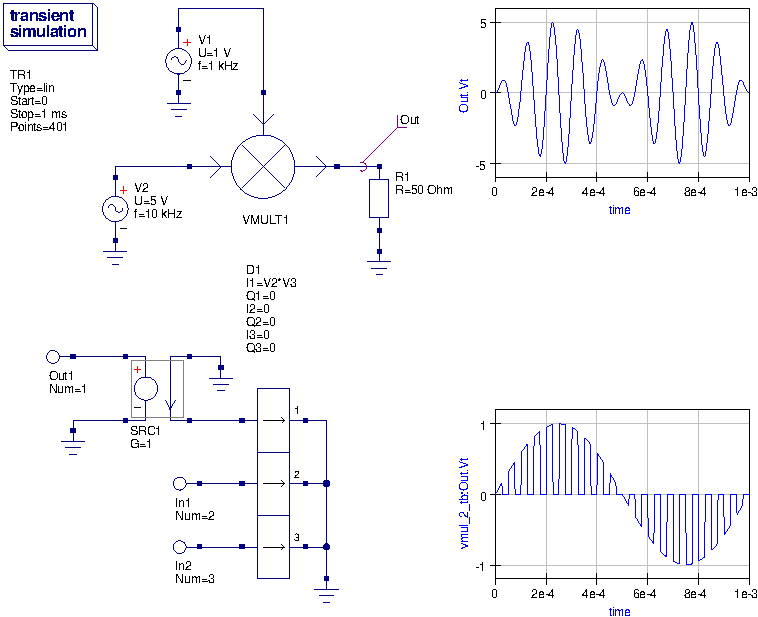
\includegraphics[width=1\linewidth]{equ_fig14}
  \caption{Qucs EDD four quadrent multiplier model and test circuit}
  \label{fig:equ_14}
\end{figure} 

\tutsection{The Qucs EDD component}

A two terminal model for a universal non-linear component with
resistive, capacitive and inductive parallel branches is shown in
Fig.~\ref{fig:equ_16}. All three branches have elements that can be
functions of either voltage or current or charge\footnote{Each branch
can be a function of one or more of these circuit variables but not
necessarily all three at the same time.}.  The Qucs EDD component can
be used to model this nonlinear device. One EDD element is needed to
model the resistive and capacitive branches. A second EDD device, plus
a gyrator, models the inductive branch.  The total terminal current is
the sum of the individual branch currents. Equations for the three
branch currents are given by the following equations:
\begin{equation}
 I=I1+IC+IL,
\end{equation}
where
\begin{equation}
I1 =f(V),\;\; IC=C(V,I)\cdot \dfrac{dV1}{dt} = \dfrac{dQ1}{dt} 
\end{equation} 
Also
\begin{equation}
  V1=i2,\;\;  V2= -IL,\;\;  i2=-L(I) \cdot \dfrac{dV2}{dt},\;\;   V1 = L(I)\cdot \dfrac{dIL}{dt}
\end{equation} 
Giving
\begin{equation}
 IL = \dfrac{1}{L(I)} \cdot \int V2\cdot dt 
\end{equation} 
and
\begin{equation}
 VL= V2 = V1 = \dfrac{d\Phi}{dt}
\end{equation} 
Hence
\begin{equation}
 I=f(V)+C(V,I)\cdot \dfrac{dV1}{dt}+\dfrac{1}{L(I)} \cdot \int V1\cdot dt
\end{equation} 

The EDD is characterised by eight parallel branches each comprising a
current component $In$ and a charge component $Qn$, where n ranges
from 1 to 8. The currents may be constants or defined by equations
that are functions of the EDD branch voltages (these are designated
$V1$ to $V8$). This form of the EDD component is known as the explicit
EDD model. Please note, EDD currents cannot be functions of
current. However, with release 0.0.12 implementation of the explicit
EDD the device charge can be a function of either voltage or
current\footnote{This allows modelling of semiconductor capacitive
effects where the amount of stored charge is either a function of
voltage (depletion layer capacitance), or a function of current
(diffusion capacitance).}. The current in the resistive branch being a
function of EDD voltage allows a range of two terminal\footnote{The
number of device terminals can be increased to model transistors and
other devices.} devices to be modelled, allowing, for example,
nonlinear resistors and diode models to be easily developed.
Similarly, the fact that the EDD charge can be a function of voltage
or current extends the range of allowed Qucs capacitor types opening
new areas of application.  The same comments apply to the nonlinear
inductors where components that have inductance values which are
functions of current allow modelling of nonlinear transformer and
coupled inductor effects. This was not possible with earlier Qucs
releases.
The EDD current and charge values may be defined by symbolic equations
that include the operators and functions listed in the ``Short
description of mathematical functions`` entry in the Qucs help
index\footnote{The Qucs operators and functions are a superset of
those defined in the Verilog-A language manual. However, in some cases
the name of the operator or function differs slightly. For example
Verilog-A uses $pow(x,y)$ for the power function whilst Qucs uses
$\wedge$ to denote $x^y$. An example of differing function names are
the inverse trigonometric functions. A list of the available functions
is given in Appendix A. }.

\begin{figure}[h]
  \centering
  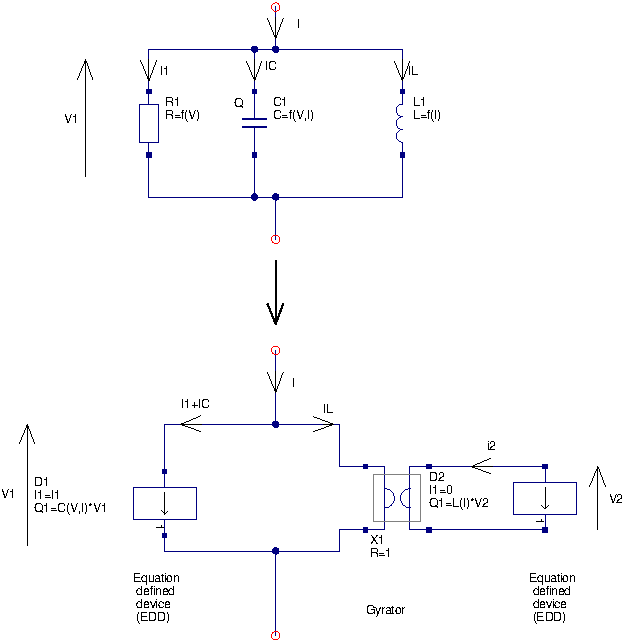
\includegraphics[width=1.0\linewidth]{equ_fig16} 
  \caption{A non-linear two terminal branch with parallel resistive, capacitive and inductive components}
  \label{fig:equ_16}
\end{figure} 

\tutsection{Modelling nonlinear resistors}

In many measurement applications a transducer is employed to transform
changing values of a physical quantity to, say, changes in resistance.
Often the resistive characterstics of these devices are nonlinear. To
demonstrate how the EDD can be used to model a nonlinear resistance
the example shown in Fig.~\ref{fig:equ_17} is introduced. In this
schematic an EDD represents a resistance that is a function of the
applied voltage across it's terminals.  This example deliberately
shows an extreme case where the resistance changes in a resistive
pulse like fashion as the terminal voltage increases. The example also
introduces for the first time the ternary ? : operator and illustrates
how it can be nested to give an ''if then else`` structure to define
the component properties. A point of note with these very nonlinear
devices centres around the fact that it is possible to define
components that have discontinuities in their I-V
characteristics\footnote{One effect of such a discontinuity is the
introduction of rapidly changing circuit conditions which can cause
the simulator difficulties in converging to a correct
solution. Sometimes, if this happens, simulation run times may be
dramatically increased or simulation fails altogether.}. The EDD
current equation defines how the resistance of this device changes
with changing terminal voltage.  This equation is given by

\begin{verbatim}
I1=V1/((V1<1.0) ? 1000 : (V1<2.0) 
                ? 1000+4000*(V1-1) : (V1<5.0) 
                ? 5000 : ((V1 >=5.0) &&  (V1<6.0)) 
                ? 5000-4500*(V1-5.0) : 500)
\end{verbatim}  

Which in terms of an ''if then else`` type statement is equivalent to:

\begin{verbatim}
I1 = V1/( if (V1 < 1.0) then 1000
          else if (V1 <  2.0) then 1000 + 4000*(V1-1)
          else if (V1 <  5.0) then 5000
          else if ((V1 >= 5.0) && (V1 < 6.0)) then 5000 - 4500*(V1-5.0)
          else 500 )
\end{verbatim} 


\begin{figure}[h]
  \centering
  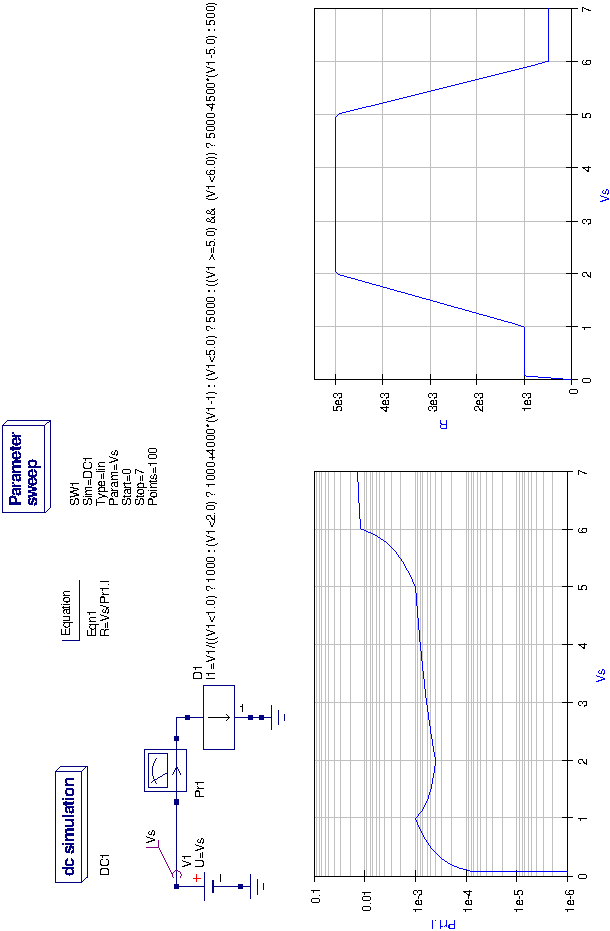
\includegraphics[width=0.8\linewidth]{equ_fig17}
  \caption{Qucs nonlinear resistor model}
  \label{fig:equ_17} 
\end{figure} 



\tutsection{Modelling nonlinear capacitors and inductors}

Nonlinear capacitors, who's C value is a function of terminal voltage,
and nonlinear inductors, who's L value is a function of terminal
current, commonly act as control elements in electronic systems. SPICE
2g6 includes a nonlinear symbolic polynomial form of C and
L\footnote{The details of these polynomial functions are presented in
Test Reports 4 and 5 of the SPICE to Qucs testing Series, Mike
Brinson, \url{http://qucs.sourceforge.net/docs.html}.}. The schematic
shown in Fig.~\ref{fig:equ_18} illustrates how a nonlinear capacitor
can be modelled by an EDD. This model is based on a SPICE like
polynomial function with four coefficients; C0, C1, C2 and
C3\footnote{SPICE 2g6 allows up to twenty coefficients. Simply add
more higher order terms to the Qucs polynomial if required.}. The test
circuit is a simple RC network with nominally identical R and C
component values to those shown in Fig.~\ref{fig:equ_2}. Increasing
the value of DC source V1 also increases C which in turn decreases the
RC low pass filter -3dB frequency. This effect is very visible in 
Fig.~\ref{fig:equ_18}. The nonlinear changes in C are also clearly
illustrated in the output voltage and phase curves. The schematic
symbol for the nonlinear capacitor is shown in Fig.~\ref{fig:equ_18}
with a red ring drawn around the normal capacitor symbol. This denotes
an EDD based component. An alternative convention is to use red
lettering within a symbol. The test circuit and simulation results for
a nonlinear inductance are shown in Fig.~\ref{fig:equ_19}. The EDD
model is similar to the SPICE 2g6 nonlinear inductance model with four 
coefficients. This number can be increased, if required, by extending
the EDD polynomial expression. A gyrator is employed with the EDD to
model the nonlinear inductance. The effect of nonlinear inductance on
the inductance current is shown by the difference between probe 
currents \textit{Pr1} and \textit{Pr2}.


 

\begin{figure}[h]   
  \centering
  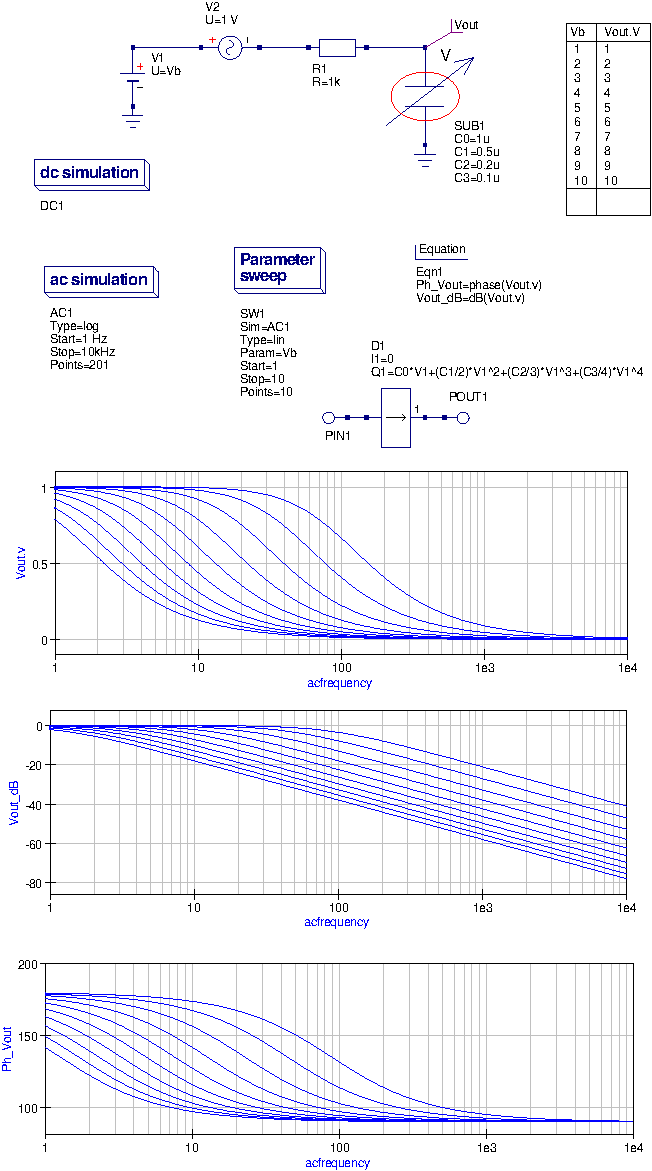
\includegraphics[width=0.7\linewidth]{equ_fig18}  
  \caption{Qucs nonlinear capacitor model} 
  \label{fig:equ_18} 
\end{figure} 

\begin{figure}[h] 
  \centering
  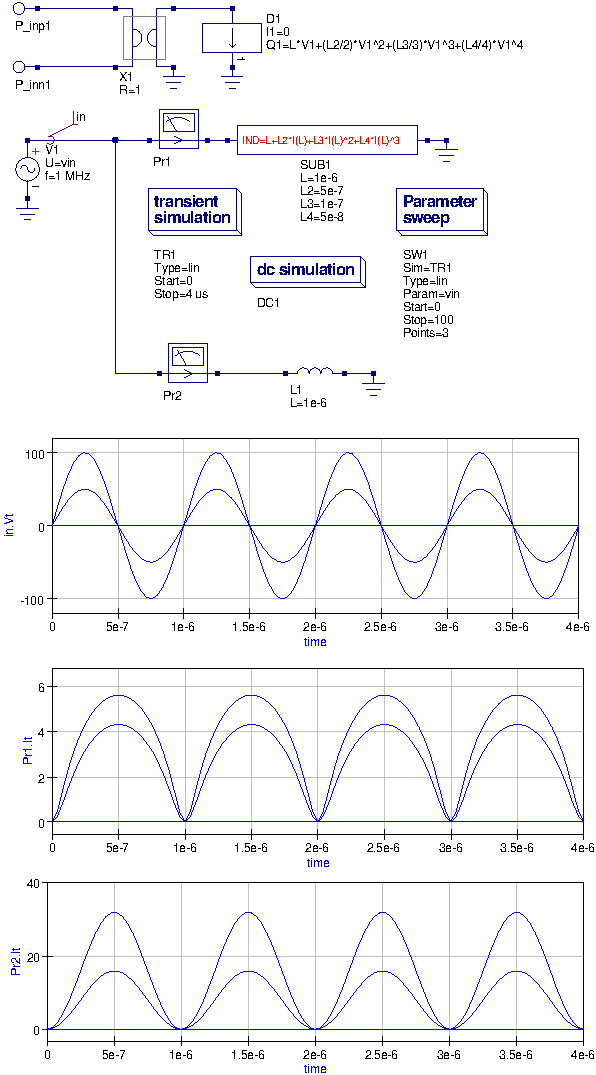
\includegraphics[width=0.7\linewidth]{equ_fig19} 
  \caption{Qucs nonlinear inductor model} 
  \label{fig:equ_19}
\end{figure} 


\tutsection{Compact device modelling using EDD}

Semiconductor device models are a corner stone of all circuit
simulators.  Often they are characterised by the same parameters as
those found in the SPICE 2g6 and 3f5 diode, BJT, FET and MOS
models.\footnote{The SPICE 2g6 and 3f5 device parameters are a subset
of those commonly provided with current generation of circuit
simulators, including Qucs.}.  Since the original SPICE semiconductor
device models where first developed many new extensions to these
models have been proposed.  Unfortunately, adding such models to a
circuit simulator is a complex process, being both time consuming and
requiring specialised knowledge. For the average Qucs user the hand
coded C++ model generation route is one that they would not
contemplate attempting because of the depth of knowledge and
specialised skills required. The Qucs EDD was devised to promote fast,
and straight forward, prototyping of semiconductor compact models,
allowing a wider Qucs population the opportunity to try their hand at
device model construction. To demonstrate the stages needed to
generate an EDD model of a semiconductor device a compact model of a
diode is introduced in this section\footnote{A second three terminal
MESFET transistor example is available for downloading from the Qucs
Web site.}.

\vspace{3mm}

The DC diode current $I_{d}$ is given by the following functions of
diode voltage $V_{d}$\footnote{These equations are for the SPICE 2g6
diode model, see Giuseppe Massobrio, Chapter 1, Pn-junction diode and
Schottky diode, Semiconductor device modeling with SPICE, Edited by
Paolo Antognetti, Giuseppe Massobrio, 1988, McGraw-Hill,Inc, ISBN
0-07-002107-4.}.


 \begin{equation}
I_{d} = I_{s}\cdot\left( \exp\left(V_{d}/(n\cdot Vt\right) -1 \right) +V_{d} \cdot GMIN,
\hspace{5mm}\forall\; (-5 \cdot n \cdot Vt \leq V_{d})
 \end{equation} 


\begin{equation}
 I_{d} = -I_{s}+V_{d}\cdot GMIN, \hspace{5mm}\forall\; (-BV <V_{d}) \hspace{2mm} \textrm{ and } \hspace{2mm} (V_{d} <-5 \cdot n \cdot Vt \leq V_{d})
\end{equation} 


\begin{equation}
 I_{d} = -IBV, \hspace{5mm}\forall\; (V_{d} = -BV)
\end{equation} 


\begin{equation}
 I_{d} = -I_{s}\cdot \left( \exp\left(-(BV+V_{d})/Vt\right)-1+BV/Vt\right), \hspace{5mm} \forall\; (V_{d } < -BV).
\end{equation} 

\vspace{3mm}

In these equations:
\begin{itemize}
 \item $I_{s}$ = the saturation current.
 \item $n$ = the emission coefficient.
 \item $GMIN$ = a small conductance in parallel with the diode\footnote{GMIN is added to help Qucs DC convergence. The SPICE default value is 1e-12S.}
 \item $Vt = kB\cdot T/q$, where $T$ is the diode temperature in Kelvin, $kB$ is Boltzmann's constant and $q$ the charge on the electron.
 \item $BV$ = reverse breakdown voltage (positive number) 
 \item $IBV$ = reverse breakdown current (positive number).
\end{itemize}

Figure~\ref{fig:equ_20} gives the EDD model for the experimental
semiconductor diode. The ternary operator ?: is used to select the
correct equation for each diode operating region. The diode current $I_d$
is the sum of EDD branch currents $I1$ to $I4$, where $I1$ represents the
diode forward bias region, $I2$ the reverse bias region and $I3$ plus $I4$
the diode reverse bias breakdown region. When calculating diode
current a special form of the exponential function exp(), called
limexp(), is employed to assist Qucs to converge to a solution during
DC and transient large signal analysis. The function limexp()
linearises the exponential function at large argument values
minimising the possibility of floating point overflow and generation
of software exceptions. The $I_{d}-V_{d}$ characteristic curves shown
in Fig.~\ref{fig:equ_20} are for the forward bias region with series
resistance $rs$ set to 0.01$\Omega$. For completeness the simulation
data for the Qucs built-in diode are also given. Clearly the two sets
of results are very similar. The DC simulation results for the diode
reverse breakdown region of operation are shown in
Fig.~\ref{fig:equ_21}. Again for comparison an $I_{d}-V_{d}$ plot for
the Qucs built-in diode is also provided. In this region of operation
some slight differences are apparent: although for both devices the
reverse breakdown is very close to 100V the slope of the $Id-Vd$ curve
at negative voltages beyond -$BV$ is different, emphasising that the
SPICE diode model does not model breakdown or zener effects
well\footnote{See Steven M. Sandler, SPICE subcircuit accurately
models zener characteristics, Personal Engineering, November 1998, pp
45-48 for more information on this subject.}.

\begin{figure} 
  \centering
  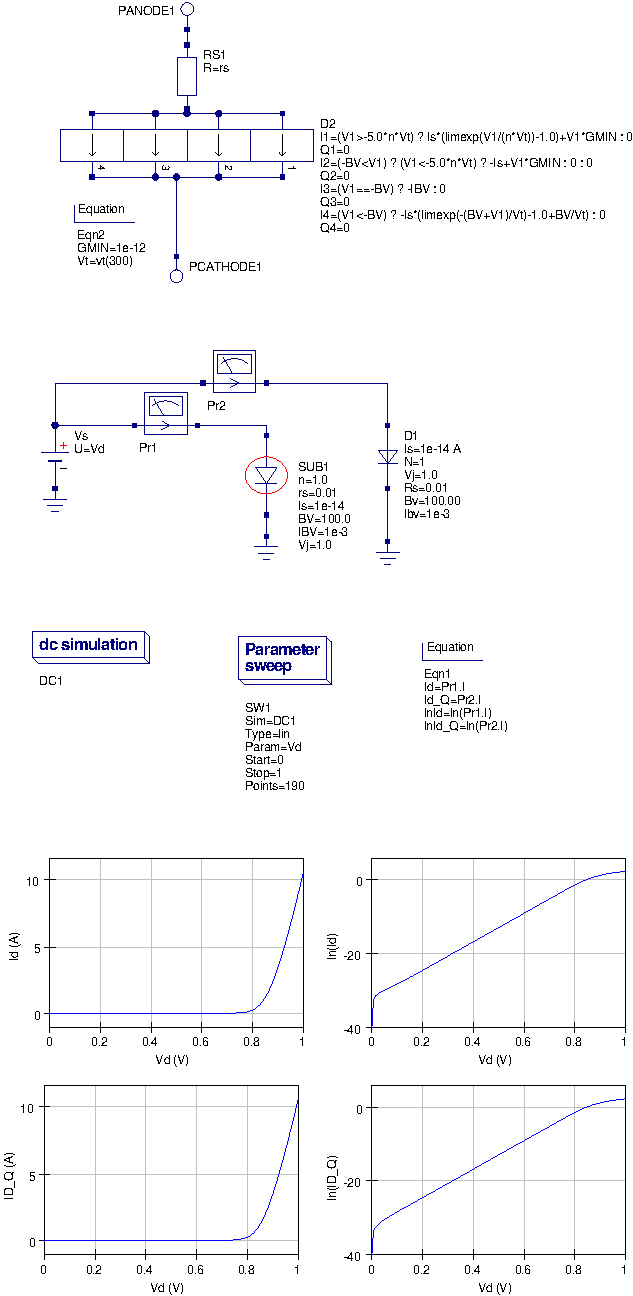
\includegraphics[width=0.63\linewidth]{equ_fig20}
  \caption{Compact diode model DC test circuit and simulation results: SUB1 is the EDD diode model and D1 the Qucs diode model with the same parameters as SUB1. } 
  \label{fig:equ_20}
\end{figure} 


\begin{figure} 
  \centering
  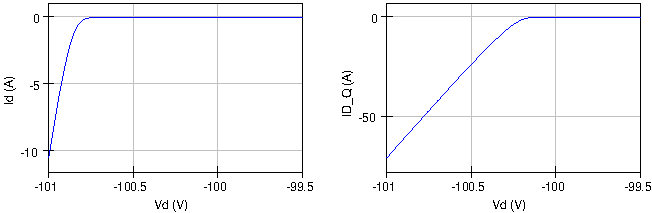
\includegraphics[width=0.63\linewidth]{equ_fig21}
  \caption{Compact diode model DC simulation results for the reverse breakdown region of operation } 
  \label{fig:equ_21}
\end{figure} 

\vspace{3mm}

The next stage in the development of the diode model is to add
capacitance effects: depletion layer capacitance for the reverse bias
region and diffusion capacitance for the forward bias region. Diode
capacitance is given by:

\begin{itemize}
 \item Depletion layer capacitance
\begin{equation}
 C_{dep} = \dfrac{dQ_{dep}}{dV_{d}} = Area \cdot Cj0\left( 1-\dfrac{V_{d}}{V_{j}}\right) ^{-m}  
\end{equation}
\item Diffusion capacitance
\begin{equation}
 C_{diff} = \dfrac{dQ_{diff}}{dV_{d}} = tt \cdot \dfrac{dI_{d}}{dV_{d}}
\end{equation} 
\end{itemize}

Where the total stored charge $Q_{d} = Q_{dep} + Q_{diff}$.  Using the same notation as the SPICE diode model:

\begin{equation}
Q_{diff} = tt \cdot I_{d}
\end{equation} 
\begin{equation}
 Q_{dep} = Area \cdot Cj0 \int\limits_{0}^{V_{d}}\left( 1-\dfrac{V_d}{V_j}\right)^{-m} dV,  \hspace{5mm} \forall\; (V_{d} <= FC \cdot V_j)
\end{equation} 

Using integration formula $\int (ax+b)^{n}dx = \dfrac{1}{a} \dfrac{\left( ax+b\right) ^{1+n}}{1+n}$ and simplifying yields:

\begin{equation}
 Q_{dep} = \dfrac{Area \cdot Cj0 \cdot V_{j}}{1-m} \left[ 1 - \left( 1-\dfrac{V_d}{V_j}\right)^{1-m}  \right]
\end{equation} 

Also, in the forward bias region 
\begin{equation}
 Q_{dep} = Area \cdot Cj0 \cdot F1 + \dfrac{Area \cdot Cj0}{F2} \int\limits_{FC \cdot V_{j}}^{V_{d}}\left( F3+\dfrac{m \cdot V_d}{V_j}\right) dV, \hspace{5mm} \forall\; (V_{d} >= FC \cdot V_j) 
\end{equation} 

On integrating

\begin{equation}
 Q_{dep} = Area \cdot Cj0 \left[ F1+\left( \dfrac{1}{F2}\right) \cdot \left\lbrace F3\cdot \left( V_{d}-FC \cdot V_{j}\right) + \left( \dfrac{m}{2 \cdot V_{j}}\right) \cdot \left( V_d^{2}+(FC \cdot V_{j})^{2}\right) \right\rbrace \right] 
\end{equation} 

Where

\begin{equation}
 F1 = \dfrac{V_j}{1-m}\left[ 1-\left( 1-FC\right) ^{1-m}\right\rbrace ,
 F2 = \left( 1-FC\right) ^{1+m},
 F3 = 1 - FC \cdot \left( 1+m\right) 
\end{equation} 


In these equations:
\begin{itemize}
 \item  $FC$ = Coefficient for forward-bias depletion capacitance.
 \item  $m $ = Grading coefficient.
 \item  $tt$ = Transit time.
 \item  $Area$ = Device area.
 \item  $Cj0$ = Zero-bias junction capacitance.
\end{itemize}

Figure~\ref{fig:equ_22m} shows the extended diode model. The $C_{dep}$ and
$C_{diff}$ components of the device capacitance have been included in the
EDD model as stored charge Q1 and Q2. Again the ternary operator ?: is
employed to select the correct equation for each section of the diode
DC operating range. An equation block is used to simplify the charge 
equations through the use of factors F1, F2 and F3.\footnote{In complex
current and charge expressions precalculating subexpressions in
equation blocks ensures that they are only calculated once at the
beginning of a simulation, ensuring minimum run times for an EDD
model.}. An area factor has also been added to the EDD model in
Fig.~\ref{fig:equ_22m}. This is introduced to allow simulation of two
or more equivalent parallel devices. The diode variables scaled by
area are:

\begin{equation}
 I_{s}(A)=I_{s} \cdot Area,\hspace{5mm} Cj0(A) = Cj0 \cdot Area, \hspace{5mm}\textrm{ and } \hspace{5mm} r_{s}(A) = rs/Area.
\end{equation} 

The test circuit shown in Fig.~\ref{fig:equ_22m} illustrates how device
capacitance and resistance can be determined as a function of diode
bias voltage. Firstly, the diode S parameters are determined at a
given bias voltage, secondly these are converted to Y parameters and
the diode capacitance ($Cap$) and resistance ($RD$) extracted from
$Y[1,1]$, and finally the variation of $Cap$ and $RD$ with diode
voltage $V_{d}$ plotted using the Qucs plotting function
PlotVs. Notice that the value of Cap at $V_{d} = 0V$ agrees with the 
value of $Cj0$.

\begin{figure} 
  \centering
  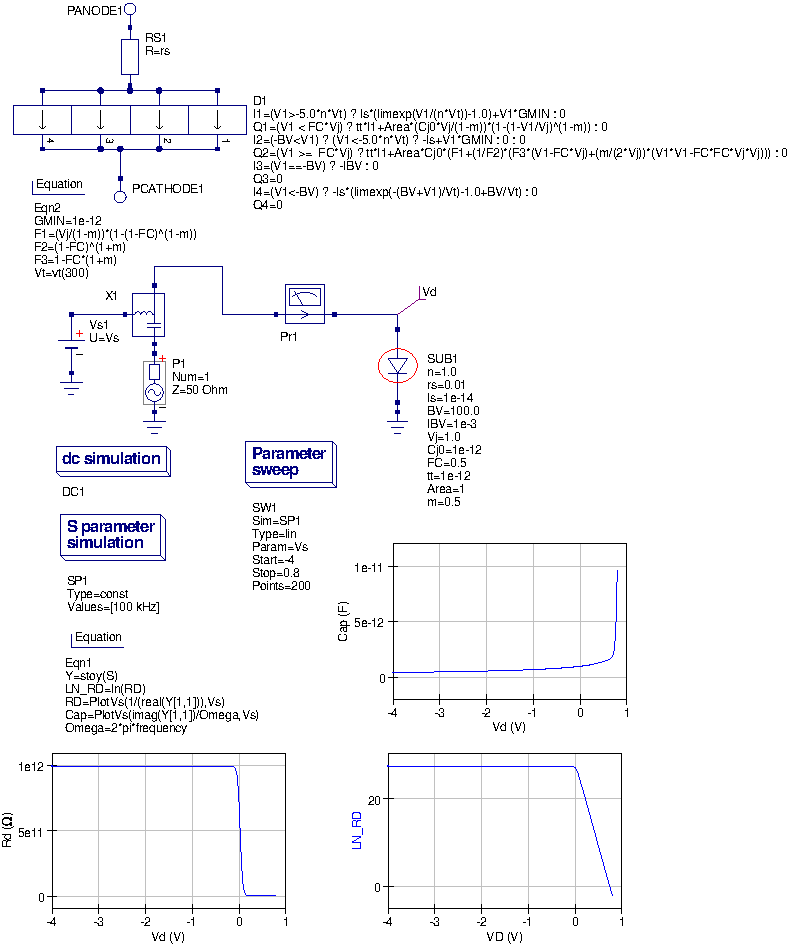
\includegraphics[width=1.0\linewidth]{equ_fig22m}
  \caption{Compact diode model capacitance and resistance simulation} 
  \label{fig:equ_22m}
\end{figure} 

\vspace{3mm}

To complete the demonstration EDD diode model all that remains to do
is to add temperature dependence to the current and capacitance
equations. Circuit simulators normally use two temperatures to
determine device temperature dependence; the first called Tnom
represents the temperature that the device parameters were measured,
and the second called Temp represents the current device
temperature. A high percentage of the diode parameters are temperature
dependent. However, to simplify the demonstration diode model only the
temperature dependence of parameters $I_{s}$, $Vj$ and $Cj0$ will be
included in the model. Adding extra temperature dependence to the
diode model is left to readers as an exercise\footnote{For example,
parameters $m$ and $BV$ are both temperature dependent.}.  One of the
great advantages of the EDD style of modelling is that it is
interactive allowing easy experimentation with models to any given
level.  The following equations list the temperature dependence of
$I_{s}$, $Vj$ and $Cj0$.

\vspace{3mm}

Let T1 = Tnom and T2 = Temp, then
\begin{equation}
 I_{s} (T2)=I_{s}(T1) \left\lbrace \dfrac{T2}{T1}\right\rbrace ^{\frac{XTI}{n}} \exp\left[ \dfrac{-q \cdot Eg(300)}{kB \cdot T2}
 \left( 1 - \dfrac{T2}{T1}\right) \right]
 \end{equation} 

\begin{equation}
 Vj (T2) = \dfrac{T2}{T1}\cdot Vj(T1) - \dfrac{2 \cdot kB \cdot T2}{q} \ln\left( \dfrac{T2}{T1}\right) ^{1.5} - \left[ \dfrac{T2}{T1}\cdot Eg(T1) - Eg(T2)\right]  
\end{equation} 

\begin{equation}
 Cj0 (T2) = Cj0 (T1)  \left[ 1+m  \left\lbrace 400\cdot 10^{-6}  \left( T2-T1\right) - \dfrac{Vj(T2)-Vj(T1)}{Vj(T1)} \right\rbrace \right]
\end{equation} 

In these equations:
\begin{itemize}
 \item $XTI$ = Saturation current temperature exponent.
 \item $Eg(T) = EG(0)-\dfrac{7.02e-4 \cdot T^{2}}{1108+T}$, the energy gap. 
\end{itemize}

Figure~\ref{fig:equ_24} shows the extended EDD for the experimental
diode model. Again the limexp() function is used in preference to the
standard exp() function in the temperature calculations listed in
equations block Eqn2. The test circuit in Fig.~\ref{fig:equ_24} sweeps
the device temperature from 20 to 80 degrees Centigrade. The graph
inlay illustrates the experimental diode current $I_{d}$ plotted as a
function of temperature. The temperature of the built-in Qucs diode is
held constant, at room temperature, and it's current $Id\_Q$ plotted as 
an overlay. The two curves cross at room temperature, indicating
identical currents at this temperature.



\begin{figure} 
  \centering
  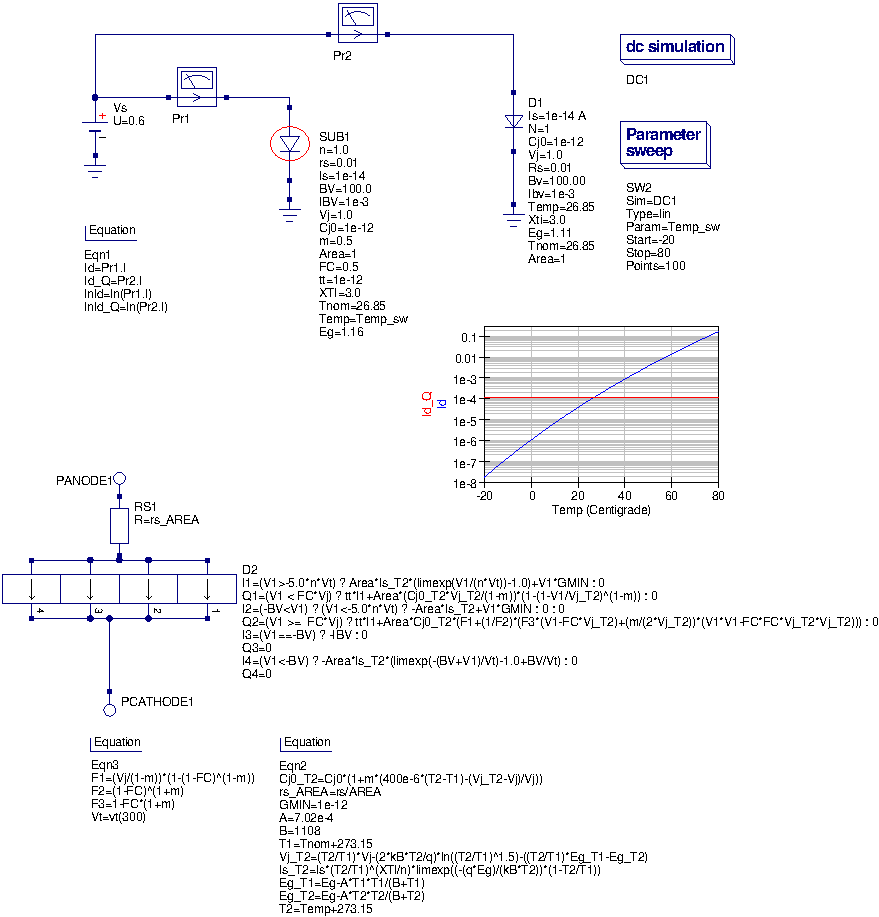
\includegraphics[width=1.0\linewidth]{equ_fig24}
  \caption{Compact diode model with temperature dependence}  
  \label{fig:equ_24}
\end{figure} 

\tutsection{Constructing EDD compact device models and circuit macromodels}

Component equations, subcircuits with parameters and EDD models are
major developments for the Qucs circuit simulator. They provide
advanced modelling capabilities with enough power and flexibility to
allow a much greater range of models to be developed than the ones
currently provided with each Qucs release. In the future it is
proposed to add new models to the Qucs Web site. The Qucs team is very
keen to encourage all Qucs users to support the modelling effort. If
you have constructed a new model and would like to share it with other
Qucs users please post your model on the qucs-devel or qucs-help
mailing lists. Both the model schematic file and a brief outline of
its operation and specification are requested.  An example model
specification for the Curtice MESFET device can be found on the Qucs
Web site. Please use the same format when writing model descriptions.

\tutsection{End Note}

This tutorial note introduces a large number of new modelling concepts
and shows how equations, subcircuits with parameters and the new
equation defined device perform a central role in constructing Qucs
models. The EDD approach to modelling makes possible, for the first
time, the construction of equation defined compact device models and
circuit macromodels using the Qucs schematic capture facilities as an
interactive modelling medium.  This is a major step forward for
Qucs. Once again these notes are very much a record of work in
progress: much still remains to be done in the future to improve the
modelling capabilities provided by Qucs. A major short term task will
be the development of additional models covering as wide a range of
applications as possible. If Qucs is to fulfill it's mission to become
a truly universal circuit simulator then it must be supported by
models.  Some readers will have noticed that these notes include very
little information about the ADMS-Verlog-A and hand coded C++ model
development routes. This was a deliberate decision on my
part. Sometime in the future I intend to return to these subjects and
update the tutorial.  A very special thank you must go to Stefan Jahn
for all his hard work, skill, and dedication during the period he has
worked on programming the amazing modelling capabilities now embedded
in Qucs.

\newpage 

\tutsection{Appendix A: Qucs constants, operators and functions}

This appendix lists the constants, operators and a number of functions
that are available for constructing Qucs equations. Items in [...]
indicate the equivalent object in the Verilog-A language. The
functions listed are common to Qucs and Verilog-A. A number of other
functions have been implemented in Qucs. The full list can be found in
the Qucs help system; ''Short Description of mathematical Functions''
or in the Qucs ''Measurement Expression Reference Manual`` by Gunther
Kraut and Stefan Jahn, \url{http://qucs.sourceforge.net/docs.html}.

\begin{itemize}
 \item Constants\begin{enumerate}
                 \item pi = 3.141593...
                 \item e  = 2.718282...
                 \item kB = 1.380651e-23 J/K
                 \item -q = -1.602177e-19 C
                \end{enumerate}
\item Operators\begin{enumerate}
                \item +x     unary plus
		\item -x     unary minus
		\item x+y    addition
		\item x-y    subtraction
		\item x*y    multiplication
		\item x/y    division
		\item x\%y   modulo (remainder)
		\item x\verb|^|y    power \hspace{2mm}[pow(x,y)]
		\item ?:     ternary  (condition) ? (expression if true) : (expression if false)
		\item ||     logical or
		\item \&\&     logical and
		\item ==     equal
		\item <      less than
		\item <=     less than or equal to
		\item >      greater than
		\item >=     greater than or equal to
		\item !=     not equal to
		\item ( )    brackets
               \end{enumerate}
\newpage 

\item Functions\begin{enumerate}
		\item ln(x)     natural logarithm
		\item log10(x)  decimal logarithm \hspace{2mm} [log(x)]
		\item exp(x)	exponential function base e
		\item sqrt(x)   square root
		\item min(x,y)  minimum
                \item max(x,y)  maximum
		\item abs(x)    absolute value
		\item sin(x)    sine
		\item cos(x)    cosine
		\item tan(x)    tangent
		\item arcsin(x) inverse sine  \hspace{2mm} [asin(x)]
		\item arccos(x) inverse cosine \hspace{2mm} [acos(x)]
		\item arctan(x[,y]) inverse tangent \hspace{2mm} [atan2(x,y)]
		\item sinh(x)   hyperbolic sine
		\item cosh(x)   hyperbolic cosine
		\item tanh(x)   hyperbolic tangent
		\item arsinh(x) inverse hyperbolic sine  \hspace{2mm} [asinh(x)]
		\item arcosh(x) inverse hyperbolic cosine \hspace{2mm} [acosh(x)]
		\item artanh(x0 inverse hyperbolic tangent \hspace{2mm} [atanh(x)]
		\item limexp(x) argument limited exponential function
		\item hypot(x,y) Euclidean distance function
		
               \end{enumerate} 

\end{itemize}



\newpage 

\tutsection{Appendix B: Constructing subcircuits with parameters}

In this appendix a series of screen dumps illustrate the sequence
needed to construct a subcircuit with parameters.  A simple series
resonance circuit has been chosen for the demonstration.

\tutsubsection{Enter the series resonance circuit and add input and output pins}

\begin{figure}[h]
  \centering
  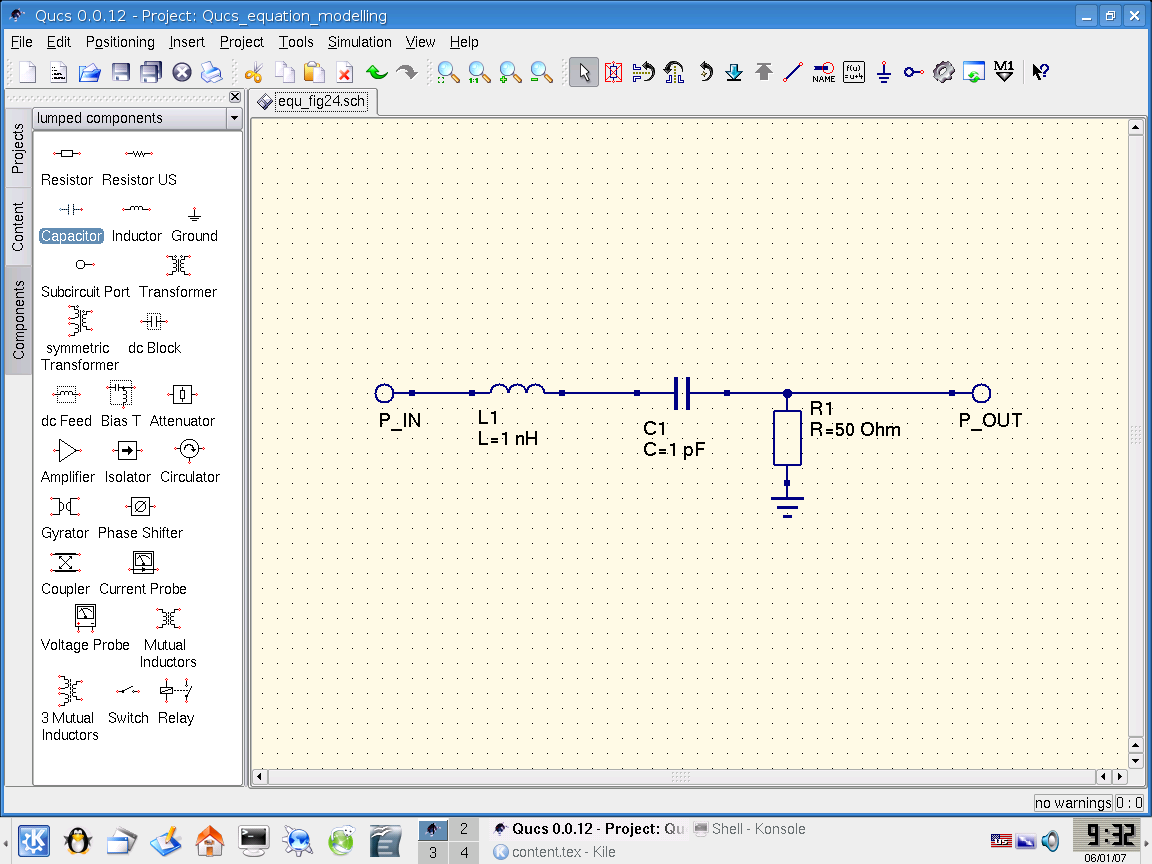
\includegraphics[width=1.0\linewidth]{equ_fig25}
  \caption{Stage 1: screen dump showing LCR circuit} 
  \label{fig:equ_25}
\end{figure} 
\FloatBarrier

\newpage 

\tutsubsection{Change the component names to Ls, Cs and Rs}

\begin{figure}[h]
  \centering
  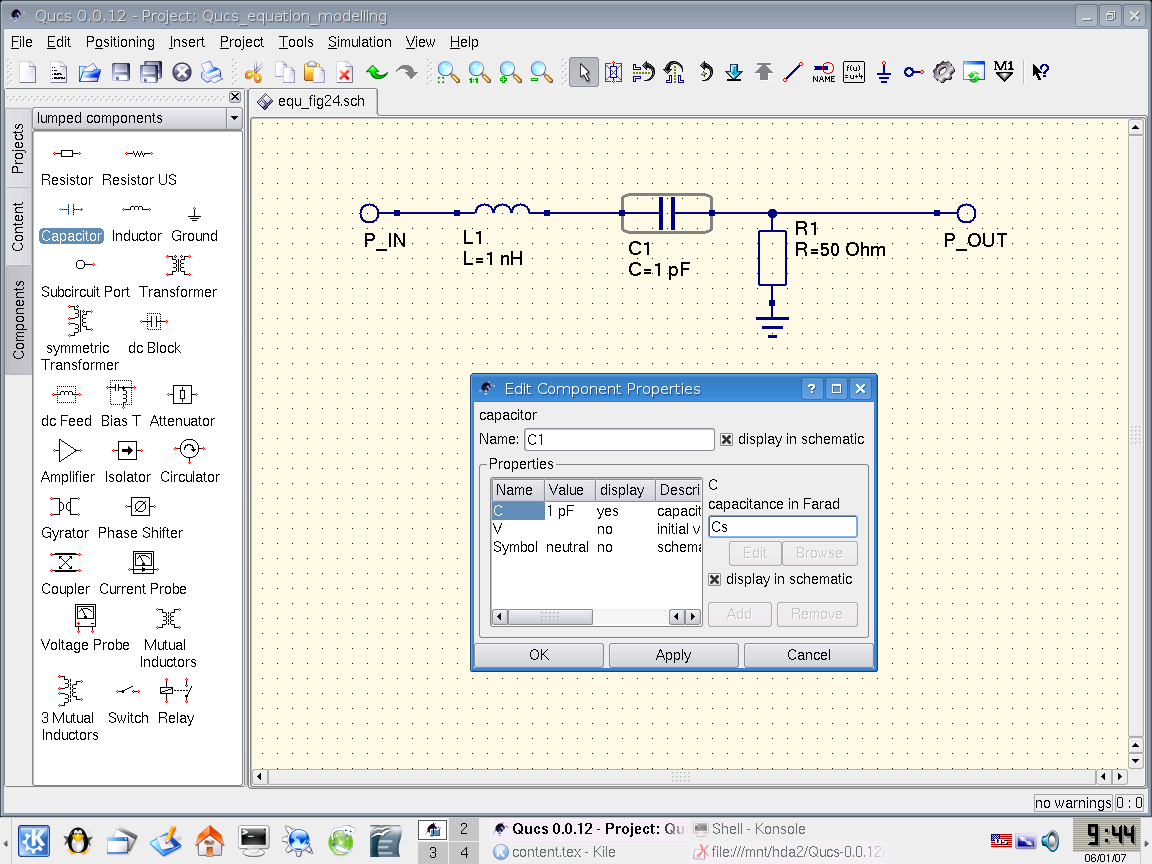
\includegraphics[width=0.56\linewidth]{equ_fig26}
  \caption{Stage 2: screen dump showing LRC circuit} 
  \label{fig:equ_26}
\end{figure} 

\begin{figure}[h]
  \centering
  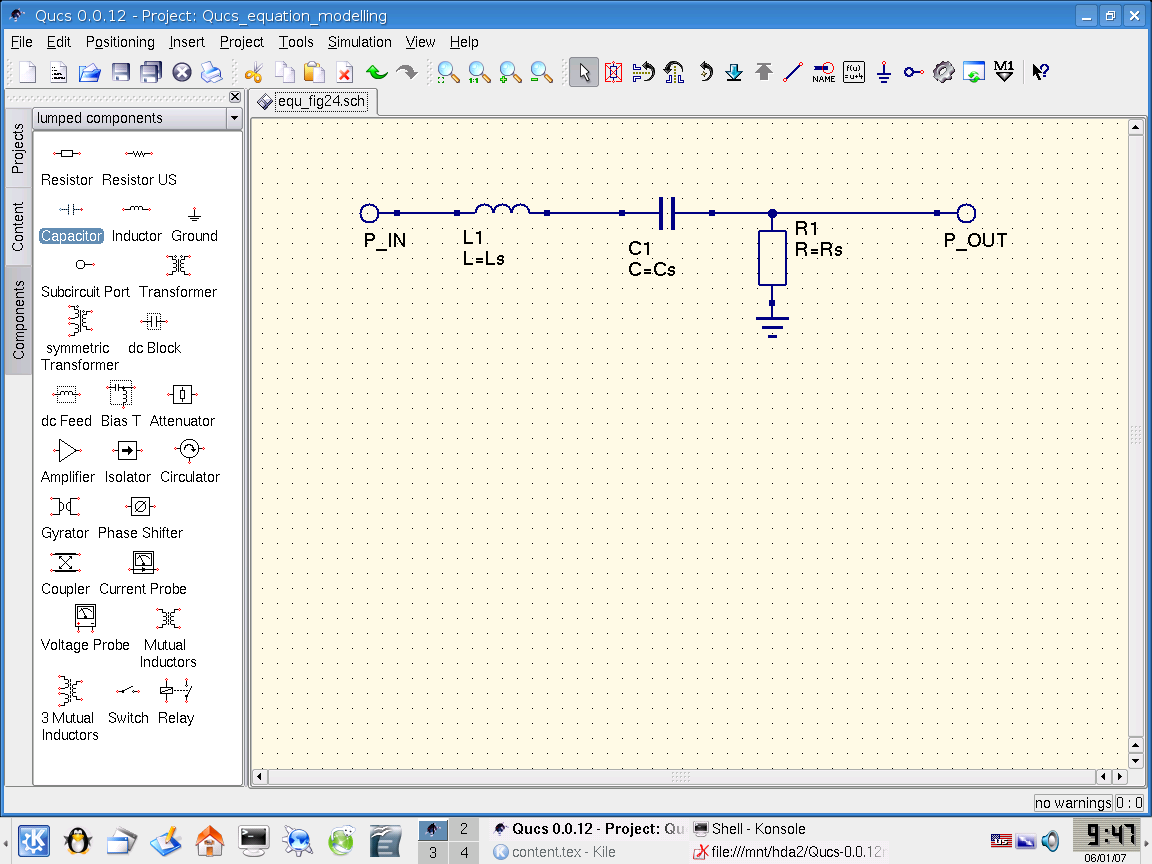
\includegraphics[width=0.56\linewidth]{equ_fig27}
  \caption{Stage 2: screen dump after name changes} 
  \label{fig:equ_27}
\end{figure} 
\FloatBarrier

\newpage 

\tutsubsection{Construct symbol for new subcircuit}

Right click on the Qucs drawing area and select Edit Circuit symbol or
press key F9. Edit the drawing symbol to give the design shown in
Fig.~\ref{fig:equ_28}.

\begin{figure}[h] 
  \centering
  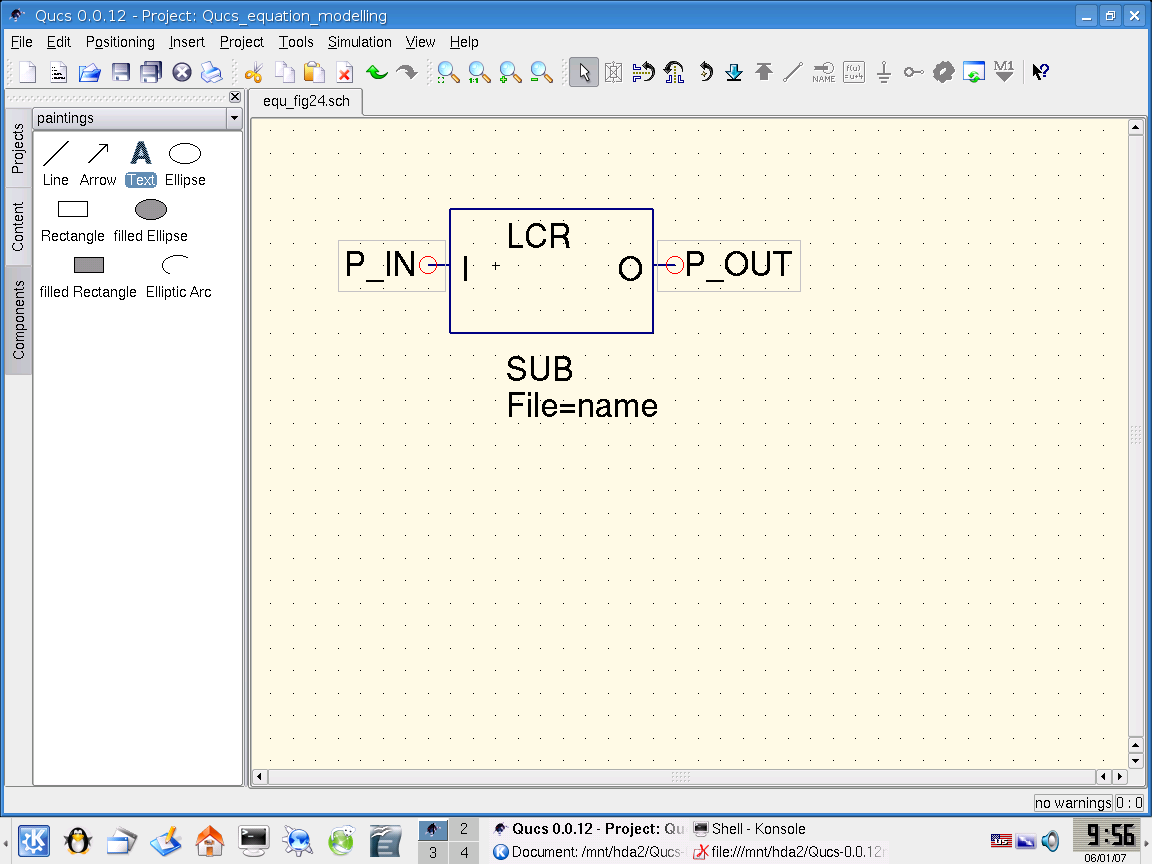
\includegraphics[width=1.0\linewidth]{equ_fig28}
  \caption{Stage 3: the subcircuit symbol} 
  \label{fig:equ_28}
\end{figure} 
\FloatBarrier

\newpage 

\tutsubsection{Add the names of the subcircuit parameters to the LCR symbol}

Right click on the SUB / File=name caption and enter names of
subcircuit parameters with their default values.

\begin{figure}[h]
  \centering
  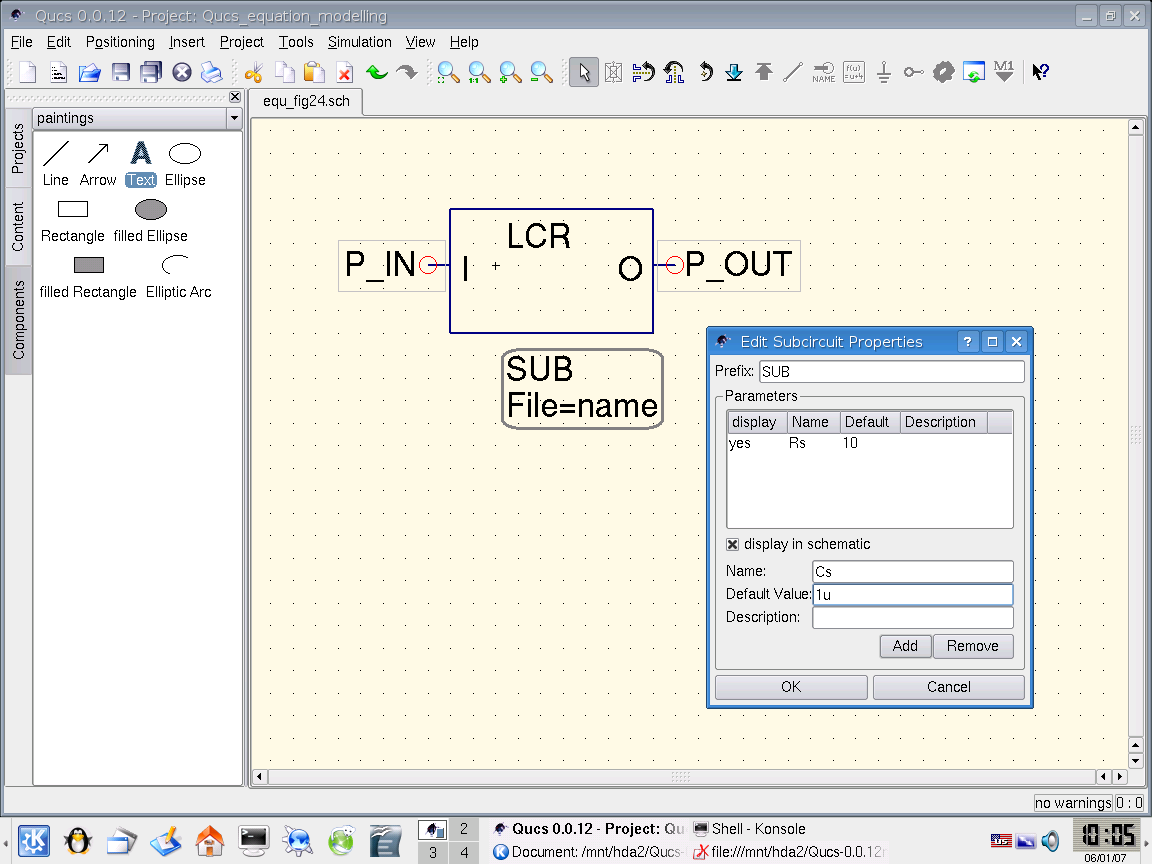
\includegraphics[width=0.53\linewidth]{equ_fig29}
  \caption{Stage 4: entering subcircuit parameter names and default values} 
  \label{fig:equ_29}
\end{figure} 

\begin{figure}[h]
  \centering
  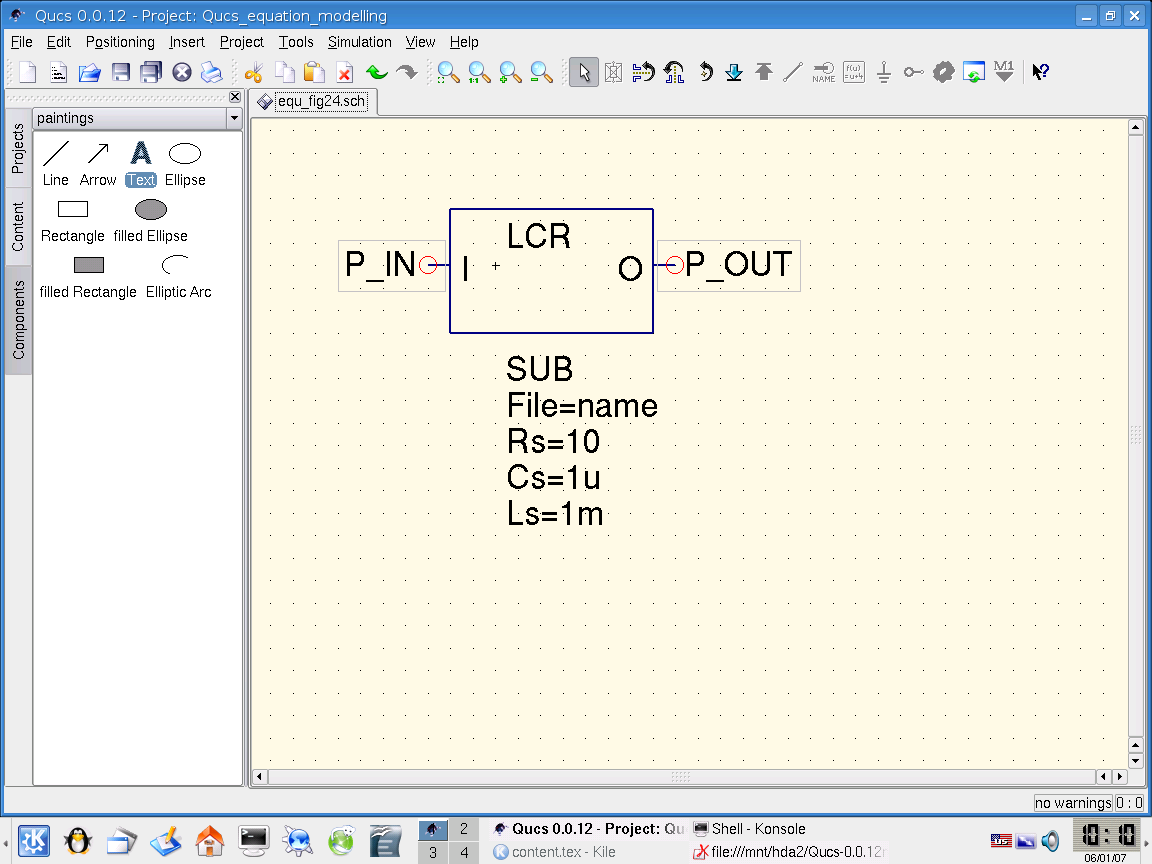
\includegraphics[width=0.53\linewidth]{equ_fig30}
  \caption{Stage 4: resulting subcircuit and parameter list with default values} 
  \label{fig:equ_30}
\end{figure} 
\FloatBarrier

\newpage

\tutsubsection{Test the LCR subcircuit}

Figure~\ref{fig:equ_31} gives a simple AC transfer function test
circuit and resulting waveforms.  Parameter \textit{R\_SW} is swept
over the range 1$\Omega$ to 10$\Omega$ and the AC transfer function
recorded and plotted.

\begin{figure}[h]
  \centering
  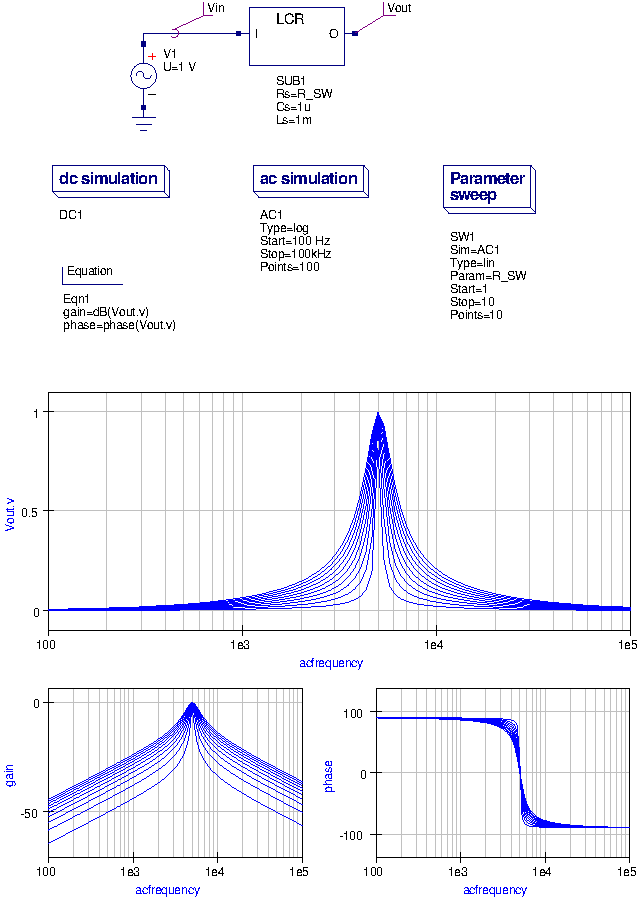
\includegraphics[width=0.7\linewidth]{equ_fig31}
  \caption{Stage 5: Subcircuit test circuit and output waveforms} 
  \label{fig:equ_31}
\end{figure} 


\tutend
